\documentclass[
    paper=A4,pagesize=automedia,fontsize=12pt,
    BCOR=15mm,DIV=22,
    twoside,headinclude,footinclude=false,
    fleqn,             % fleqn = linksbündige Ausrichtung von Formeln
    bibliography=totocnumbered,          % Literaturverz. im Inhaltsverz. eintragen
    listof=totoc,                % Abbildungsverz. im Inhaltsverz. eintragen
    listof=flat,                 % Abbildungsverz. an der längsten Nummer ausrichten
    cleardoublepage=empty      % Vakatseiten ohne Paginierung
    numbers=endperiod
]{scrartcl}
\setlength\parindent{0em}

\usepackage{hyperref}
\hypersetup{
    colorlinks=false, %set true if you want colored links
    linktoc=all,     %set to all if you want both sections and subsections linked
    linkcolor=blue,  %choose some color if you want links to stand out
}

% Kodierung, Schrift und Sprache auswählen
\usepackage[utf8]{inputenc}
\usepackage[T1]{fontenc}
\usepackage[english]{babel}
% damit man Text aus dem PDF korrekt rauskopieren kann
\usepackage{cmap}
% Layout: Kopf-/Fußzeilen, anderthalbfacher Zeilenabstand
\usepackage[headsepline]{scrlayer-scrpage}
\pagestyle{scrheadings}
\clearpairofpagestyles
\ihead{\headmark}
\ohead{\pagemark}
\automark[subsection]{section}
\KOMAoption{headsepline}{0.5pt}

\usepackage{setspace}
\onehalfspacing
\deffootnote{1em}{1em}{\textsuperscript{\thefootnotemark}}

% Grafiken, Tabellen, Mathematikumgebungen
\usepackage{graphicx,xcolor}
\usepackage{tabularx}
\usepackage{amsmath,amsfonts,amssymb}

% Darstellung von Fließumgebungen
\usepackage{flafter,afterpage}
\usepackage[section]{placeins}
\usepackage[margin=8mm,font=small,labelfont=bf,format=plain]{caption}
\usepackage[margin=8mm,font=small,labelfont=bf,format=plain]{subcaption}

% \numberwithin{equation}{chapter}
% \numberwithin{figure}{chapter}
% \numberwithin{table}{chapter}

%%%%%%%%%%%%%%%%%%%%%%%%%%%%%%%%%%%%%%%%%%%%%%%%%%%%%%%%%%%%%%%%%%%%%%%%%%%%%%%%
% Ab hier ist Platz für eigene Ergänzungen (Pakete, Befehle, etc.)

% Dieses Paket liefert den Blindtext, der als Platzhalter in den Beispieldateien steht.
% Das kannst Du also entfernen, wenn Du den Blindtext nicht mehr brauchst.
\usepackage{lipsum}

\usepackage{booktabs}

\usepackage[outputdir=out]{minted}
\usemintedstyle{vs}

\graphicspath{ {./img/} }

\begin{document}

% \frontmatter

% Commands
\newcommand{\E}[1]{\langle#1\rangle}

% Titelpageseite
\begin{titlepage}
    \begin{tabularx}{\linewidth}{X}
        
\includegraphics[width=6cm]{TU_Logo_SW} \\\hline\hline

        \vspace{4.5em}

        \begin{singlespace}\begin{center}\bfseries\Huge

            Molecular dynamics study of ideal polymer chains with different persistence lengths

            \end{center}\end{singlespace}

        \vspace{5.5em}

        \begin{singlespace}\begin{center}\large
                Bachelor-Arbeit \\ zur Erlangung des Hochschulgrades \\
                Bachelor of Science \\
                im Bachelor-Studiengang Physik
            \end{center}\end{singlespace}\medskip

        \begin{center}vorgelegt von\end{center}
        \begin{center}
            {\large Yahor Paromau} \\ geboren am 29.12.1998 in Hrodna
        \end{center}\medskip

        \begin{singlespace}\begin{center}\large
                Leibniz-Institut für Polymerforschung Dresden e. V. \\
                Fakultät Physik \\
                Bereich Mathematik und Naturwissenschaften \\
                Technische Universität Dresden \\ 2023
            \end{center}\end{singlespace}
    \end{tabularx}
\end{titlepage}


% Gutachterseite
\thispagestyle{empty}\vspace*{48em}

Eingereicht am xx.~Monat~20xx\vspace{1.5em}
\par{\large\begin{tabular}{ll}
        1. Gutachter: & Prof.~Dr.~XX \\
        2. Gutachter: & Prof.~Dr.~YY \\
    \end{tabular}}


% Abstractseite
\newpage
\begin{center}\large\bfseries Summary\end{center}


Abstract \\
Utilizing molecular dynamics simulations, it is explored whether changes 
in the mechanical properties of the polymer chain, such as 
stiffness and friction coefficient of a terminal bead, may contribute to the 
observed by Singh \emph{et. al} \cite{Singh:2022} alterations in scaling behavior. 
Additionally, while the dynamics of free chains have been studied extensively 
\cite{Nikoubashman2016} \cite{Singh:2022}, 
the dynamics of anchored semiflexible chains, as observed in the process of 
membrane tethering, remain relatively unexplored. This work aims to investigate 
the dynamical properties of anchored semiflexible chains while varying their 
stiffness and terminal bead radius. This study is conducted within the 
framework of ideal chain models, 
excluding hydrodynamic interactions. Results of this study reveal insights 
into the influence of chain stiffness and friction coefficient of the chain end
on the dynamical properties of the chain in solution and provide 
valuable considerations for future research in this field.


\vspace{15em}
Kurzzusammenfassung \\
Mithilfe von Molekulardynamiksimulationen wird in dieser Studie untersucht, 
ob Veränderungen der mechanischen Eigenschaften einer Kette, 
wie Steifigkeit und Reibungskonstante des Endmonomers, 
zu den beobachteten Veränderungen im Skalierungsverhalten beitragen, 
wie sie von Singh \emph{et al.} \cite{Singh:2022} festgestellt wurden. 
Zusätzlich dazu, während umfangreiche Forschung zur Dynamik freier Ketten 
durchgeführt wurde, bleiben die Dynamik von verankerten semiflexiblen Ketten, 
wie sie beim Prozess des Membrantetherings beobachtet werden, 
vergleichsweise unerforscht. Diese Arbeit zielt darauf ab, die dynamischen 
Eigenschaften von verankerten semiflexiblen Ketten zu untersuchen, 
während ihre Steifigkeit und Reibungskonstante des Endmonomers der Endperle 
variiert werden. Die Studie erfolgt im Rahmen von Modellen idealer Ketten und schließt 
hydrodynamische Wechselwirkungen aus. Die Ergebnisse geben Einblicke in den 
Einfluss der Kettensteifigkeit und des Reibungskoeffizienten des Kettenendes auf 
ihre dynamischen Eigenschaften und liefern wertvolle Überlegungen für 
zukünftige Forschung in diesem Bereich.
% Inhaltsverzeichnis

\cleardoublepage

\thispagestyle{empty}
\tableofcontents

\cleardoublepage



\section{Introduction}
\subsection{Motivation and goal}
Intracellular traffic constitutes a intricate interplay of both mechanical 
and chemical processes starting from formation of vesicle proceeding with 
its movement along the cytoskeletal tracks ending with tethering and merging
with their corresponding target membrane compartment \cite{Singh:2022}.
Membrane tethering process, in some cases driven by the pairing of
small GTPases with long dimeric coiled-coil tether molecules, \cite{Singh:2022}  
is the coupling of chemistry with mechanics, which is not yet well 
understood \cite{Singh:2022}. There are recent discussions in the literature
about the role of the long dimeric coiled-coil molecules in the process
of overcoming the distance barriers that physically separate 
membranes \cite{Singh:2022}. Specifically, the process of membrane tethering was
obseved, driven by the conformational changes of the early endosomal
tether EEA1, caused by its binding to the small GTPase Rab5 \cite{Murray2016}.
The conformational changes of EEA1 upon the binding of Rab5 are then closely
studied by the Singh \emph{et al.} \cite{Singh:2022}. 
Among others they observed 
a change in the scaling behavior of the mean squared displacement of 
chains end upon the binding of the Rab5. They also have shown \emph{indirectly} 
that this change is caused by the stiffness transition of the chain.
However, the underlying molecules constitute a complex biological system, and
there might be other factors affecting the change in the scaling behavior.
With the help of coarse grained molecular dynamics simulations it is possible
to investigate, if such change in the dynamical properties of the chain could 
be caused by the change of mechanical properties of the chain, such as stiffness and 
friction coefficient of the chain end, 
which is increased upon the binding of Rab5. Also, while the dynamical
properties of free chains were already considered in various studies 
(among others: \cite{Singh:2022} \cite{Nikoubashman2016} 
\cite{Kremer_ChemPhys} \cite{Hinczewski_2009}), the dynamics of anchored
semiflexible chains
(as they occur in the process of membrane terhering, anchored to the endosome)
is not yet well studied. 
\\
\\
The goal of this work is, on the one hand, to study 
the dynamical properties of the anchored semiflexible chains by varying 
stiffness and 
friction of the chain end, on the other hand, to explore, if the above mentioned
mechanical properties of the free chain can cause the change in scaling behavior
of the chain, as observed in Singh \emph{et al.} \cite{Singh:2022}. The scope
of this work is limited by considering only ideal chain models and excluding
hydrodynamic interactions.


\subsection{Ideal polymer chain models}

In the realm of polymer physics, ideal chain models serve as crucial tools
for understanding the fundamental properties and behavior of polymer chains. 
These models provide simplified yet insightful descriptions of polymer chains' 
static properties and are integral to elucidating phenomena such as
polymer persistence length and overall chain behavior.
Ideal models are characterized by distinct assumptions concerning the 
permissible ranges of torsion and bond angles. Nevertheless, all 
these models disregard interactions between monomers that are widely 
spaced along the chain.
In this section, 3 relevant ideal chain models are described: 
the freely jointed chain model, freely rotating chain model and the worml-like chain model.

\paragraph{Freely jointed chain model}
The freely jointed chain model is one of the simplest chain models. It assumes
a constant bond length $l_b$ \cite{Rub_Colby_PolyPhy:2005} and no correlations between the directions of different
bond vectors \cite{Rub_Colby_PolyPhy:2005}: $\E{cos(\theta_{ij})} = 0$ for $i \neq j$. This model is suitable
to study static properties of fully flexible polymer chains. In particular interest
are the end-to-end distance of the chain with $N$ bonds
\begin{equation}
    \E{R^2} = N l_b^2
\end{equation}
and the contour length 
\begin{equation}
    L = N l_b
\end{equation}

\paragraph{Freely rotating chain model}
To define the polymer stiffness one needs to consider the polymer chain model
where correlation between bond vectors does not vanish.
The freely rotating chain (FRC) model is a fundamental ideal chain model 
that offers a simple yet valuable perspective on polymer behavior. 
This model assumes a constant bond length $l_b$ \cite{Rub_Colby_PolyPhy:2005}, 
bond angles are constant \cite{Rub_Colby_PolyPhy:2005} and
all torsion angles are equally likely and independent of each other \cite{Rub_Colby_PolyPhy:2005}.
In this model there is a correlation between bond vectors \cite{Rub_Colby_PolyPhy:2005}:
\begin{equation}
    \E{\vec{r}_i \vec{r}_j} = l_b^2 (\cos(\theta))^{|j-i|}
\end{equation}
A persistence segment of the chain is defined by the number of main-chain bonds $s_p$ 
it contains \cite{Rub_Colby_PolyPhy:2005}. This represents a scale at which local 
correlations between bond vectors decay \cite{Rub_Colby_PolyPhy:2005}.
\begin{equation}
    s_p = - \frac{1}{\ln(\cos(\theta))}
\end{equation}
The persistence length $l_p$ of the chain is then defined as \cite{Rub_Colby_PolyPhy:2005}:
\begin{equation}
    l_p = l_b s_p
\end{equation}
And the Kuhn length $l_K$ of the chain is defined as \cite{Rub_Colby_PolyPhy:2005}:
\begin{equation}
    l_K = 2 l_p
\end{equation}

\paragraph{Worm-like chain model}
The worm-like chain model is a special case of freely rotating chain model for
the small values of a bond angle: $\theta \ll 1$ \cite{Rub_Colby_PolyPhy:2005}.
It is suitable for the description of very stiff polymers \cite{Rub_Colby_PolyPhy:2005}.
In this model the number of main-chain bonds in persistence segment simplifies to 
\begin{equation}
    s_p \approx \frac{2}{\theta^2}
\end{equation}
The end-to-end distance of the chain can be written as:
\begin{equation}
    \E{R^2} = 2 l_p L - 2 l_p^2 (1-\exp(-\frac{L}{l_p}))
\end{equation}
And the following relation holds between persistence length and angles of the chain:
\begin{equation} \label{eq:worm-like-chain-cos-theta-ij}
    \E{cos(\theta_{ij})} = exp(-\frac{l_b |j-i|}{l_p})
\end{equation}
which is usefull if one needs to estimate the persistence length from the chain angles.

\subsection{Langevin equation} \label{section:langevin_eq}
The discussion of chain dynamics should start from the description of
the dynamics of single particle. This can be done using the Langevin equation. 
The Langevin equation is a fundamental stochastic differential equation 
widely used in statistical mechanics and molecular dynamics to describe the 
dynamics of particles or molecules subjected to random forces in a 
dissipative medium. Specifically Langevin equation is used to describe the 
particle in immobile solvent and can be written as:
\begin{equation} \label{eq:langevin}
    m \ddot{\vec{r}} = - \nabla U(\vec{r}) - \sigma m \dot{\vec{r}} + \vec{f}^r(t)
\end{equation}
where:
\begin{itemize}
    \item $\sigma$ - damping constaint, which accounts for the viscosity of the solvent
    \item $\vec{f}^r(t)$ - stochastic force, represents the effect of thermal 
    fluctuations due to the particle's interactions with the solvents molecules
    \item $U(\vec{r})$ - any external potential acting on the particle
\end{itemize}
$\vec{f}^r(t)$ is a stochastic process known as white noise:
\begin{itemize}
    \item Sampled from Gaussian distribution
    \item $\E{\vec{f}^r(t)} = 0$
    \item $\E{\vec{f}_{\alpha}^r(t) \vec{f}_{\beta}^r(t')} = 2 k_B T \sigma m \delta(t-t')$ which relates strength
     of noise and friction and
    is known as fluctuation-dissipation theorem.
\end{itemize}
The solution of this equation depends of course on the selected external
potential $U(\vec{r})$. In case of harmonic spring potential 
$U(\vec{r})=\frac{1}{2} k r^2$ the formal solution can be written as:
\begin{equation}
    \vec{r}(t)=\frac{1}{\zeta}\int_{-\infty}^{t} dt' \exp\left(-\frac{t-t'}{\tau}\right)\vec{f}^r(t')
\end{equation}
with $\zeta=m \sigma$ and $\tau := \zeta / k$.

\subsection{Rouse model}
Polymer chains, composed of repeating monomer units, exhibit complex 
behaviors that are of great interest in polymer physics and materials science. 
Understanding the dynamics of polymer chains is crucial for elucidating their 
mechanical, thermal, and transport properties. One of the fundamental 
models used to describe polymer dynamics is the Rouse model.
\\
\\
The Rouse model is a widely used theoretical framework to study the dynamics 
of polymer chains in an ideal solvent. This model simplifies the complex 
behavior of polymer chains by representing them as linear chains of connected beads.

\subsubsection{Flexible chain}
Firstly Rouse model for flexible free chains is introduced.
\paragraph{Assumptions}
The Rouse model makes certain key assumptions to facilitate its analytical treatment:
\begin{enumerate}
    \item \label{rouse_assumption_1} No hydrodynamic interactions or excluded volume effects between monomers.
    \item \label{rouse_assumption_2} Thermal forces acting on each bead follow Gaussian statistics.
    \item \label{rouse_assumption_3} Overdamped motion of the bead, which implies that inertia term vanishes: $m \ddot{\vec{r}} \approx 0$.
    Which is usually fulfilled in polymeric systems \cite{Doi_Intro_PP:2005}.
    \item \label{rouse_assumption_4} Beads continuously distributed along polymer chain.
\end{enumerate}

\paragraph{Equation}
Assumptions \ref{rouse_assumption_1}, \ref{rouse_assumption_2} lead to description of the
system using Langevin equation (Eq. \ref{eq:langevin}). Following assumption \ref{rouse_assumption_3} 
the inertia term is set to 0. The continous approximation then made as consequence of assumption \ref{rouse_assumption_4}.
The initial equation of motion of single bead then becomes a diffusion equation \cite{Rub_Colby_PolyPhy:2005}:
\begin{equation}
    \label{eq:diffusion}
    \zeta \frac{\partial \vec{r}(t,n)}{\partial t} = \frac{3 k_B T}{l_b^2} \frac{\partial \vec{r}(t,n)}{\partial n^2} + \vec{f}^r(t)
\end{equation}
with friction coefficient $\zeta = \sigma m$.

\paragraph{Boundary conditions}
The chain ends are connected to one spring only. These free ends could be modelled by adding two 
fictious beads to both ends with $\vec{r}_0=\vec{r}_1$ and $\vec{r}_N=\vec{r}_{N+1}$. Boundary 
conditions for diffusion equation can be then written as follows \cite{Rub_Colby_PolyPhy:2005}:
\begin{equation}
    \label{eq:rouse_boundary}
    \begin{aligned}
        & \left(\frac{\partial \vec{r}}{\partial n}\right)_{n=0} = 0\\
        & \left(\frac{\partial \vec{r}}{\partial n}\right)_{n=N} = 0
    \end{aligned}
\end{equation}

\paragraph{Solution}
The motion of the polymer can be decoupled in the motion of the independent modes using normal
coordinates \cite{Doi_Edwards_PD:1994}. Define:
\begin{equation}
    \label{eq:rouse_mode}
    \vec{X}_p := \frac{1}{N} \int_0^N dn \cos(\frac{p \pi n}{N})\vec{r}(n, t)
\end{equation}
Eq. \ref{eq:diffusion} can be then rewritten as \cite{Doi_Edwards_PD:1994}:
\begin{equation}
    \zeta_p \frac{\partial}{\partial t} \vec{X}_p = -k_p \vec{X}_p + \vec{f}^p
\end{equation}
with 
\begin{equation}
    \zeta_0 = N \zeta
    \text{ and }
    \zeta_p = 2 N \zeta
    \text{ for } p = 1,2,\ldots
\end{equation}
\begin{equation}
    k_p = \frac{6 \pi^2 k_B T}{Nl^2} p^2
    \text{ for } p = 0,1,2,\ldots
\end{equation}
and $\vec{f}^p$ is a random force, which satisfies \cite{Doi_Edwards_PD:1994}:
\begin{equation}
    \begin{aligned}
        & \E{f_{p\alpha}} = 0\\
        & \E{f_{p\alpha}(t) f_{p\beta}(t')} = 2 \delta_{pq} \delta_{\alpha\beta} \zeta_p k_B T \delta(t-t')
    \end{aligned}
\end{equation}
Which is langevin equation for the harmonic spring potential, with formal solution \cite{Doi_Edwards_PD:1994}:
\begin{equation}
    \vec{X}_p(t) = \frac{1}{\zeta_p} \int_{-\infty}^{t} dt' \frac{\exp(t-t')}{\tau_p} \vec{f^p}
\end{equation}
with
\begin{equation}
    \tau_p = \zeta_p / k_p
\end{equation}

$\vec{X}_p$ represents the local motion of the chain which includes $\frac{N}{p}$ segments and corresponds to the
motion with the length-scale of the order $\sqrt{Nl_b^2/p}$ \cite{Doi_Edwards_PD:1994}.
\\
\\
The inverse transformation of Eq. \ref{eq:rouse_mode} is given by \cite{Doi_Edwards_PD:1994}:
\begin{equation}
    \vec{r}_n = \vec{X_0} + 2 \sum_{p=1}^{\infty} \vec{X}_p \cos(p \pi n  / N)
\end{equation}

\paragraph{Relevant observables}
In this paragraph the relevant dynamical quantities of rouse model are summarized.
\\
\\
Rouse relaxation time:
\begin{equation} \label{eq:rouse_relaxation_time}
    \tau_R := \tau_1 = \frac{1}{3 \pi^2} \frac{N^2 l_b^2 \zeta}{k_B T} 
\end{equation}
matches (except of factor $1/3\pi^2$) the time needed for the chain to diffuse over it's End-to-End distance.
\\
\\
Relaxation time of the single monomer:
\begin{equation}
    \tau_0 = \frac{3 \pi^2 \tau_R}{N^2} = \frac{l_b^2 \zeta}{k_B T}
\end{equation}
matches the time needed for free particle of size $l$ to diffuse over distance
of it's own size, as described by Langevin equation for free particle.
\\
\\
Time correlation of End-to-End (ETE) vector \cite{Doi_Edwards_PD:1994}:
\begin{equation}
    \E{\vec{R}(t)\vec{R}(0)} = Nl_b^2 \sum_{p=1,3,\ldots} \frac{8}{p^2\pi^2}\exp(\frac{-t p^2}{\tau_R})
\end{equation}
with following asymptotic behavior \cite{Nikoubashman2016}:
\begin{equation}
    \E{\vec{R}(t)\vec{R}(0)} = Nl_b^2 \begin{cases}
        \frac{8}{\pi^2} \exp(\frac{-t}{\tau_R}) & \text{if } t \gg \tau_R \\
        1 - \sqrt{8t/(\pi^3\tau_R)} & \text{if } t \ll \tau_R
    \end{cases}
\end{equation}
\\
\\
Mean square displacement (MSD) of ETE:
\begin{equation} \label{eq:rouse_msd_ete}
    \begin{aligned}
        \E{[\Delta \vec{R}(t)]^2} :&= \E{[\vec{R}(t)-\vec{R}(0)]^2} \\
        & = 2\E{R^2} - 2 \E{\vec{R}(t)\vec{R}(0)} \\
        & = 2 N l_b^2 (1 - \frac{8}{\pi^2}\sum_{p=1,3,\ldots}\frac{1}{p^2} \exp(\frac{-tp^2}{\tau_R}))
    \end{aligned}
\end{equation}
with asymptotic behavior:
\begin{equation}
    \E{[\Delta \vec{R}(t)]^2} = 2Nl_b^2 \begin{cases}
        (1-\exp(\frac{-t}{\tau_R})) & \text{if } t \gg \tau_R \\
        \sqrt{8t/(\pi^3\tau_R)} & \text{if } t \ll \tau_R
    \end{cases}
\end{equation}
Also, the one can see that the scaling behavior of $\E{[\Delta \vec{R}(t)]^2}$ is given
by the scaling behavior of $\E{\vec{R}(t)\vec{R}(0)}$ and corresponding
scaling exponent is $\alpha = \frac{1}{2}$.
\\
\\
MSD of chain end (MSDLM) \cite{svaneborg_2020}:
\begin{equation}
    \E{[\Delta \vec{r}_N(t)]^2} = \frac{2}{\pi^2} \E{R^2} \left( \sum_{p=1}^{\infty} \frac{1}{p^2} \left[ 1-\exp(\frac{-t p^2}{\tau_R}) \right] + \frac{t}{\tau_R} \right)
\end{equation}
with following asymptotic behavior \cite{svaneborg_2020}:
\begin{equation}
    \E{[\Delta \vec{r}_N(t)]^2} = N l_b^2 \begin{cases}
        (\frac{1}{3} + \frac{2t}{\pi^2 \tau_R}) & \text{if } t \gg \tau_R \\
        \frac{2}{\pi^{3/2}} \sqrt{\frac{t}{\tau_R}} & \text{if } t \ll \tau_R
    \end{cases}
\end{equation}

\subsubsection{Semiflexible chain}
\label{sec:rouse_semiflex_chain}
The Rouse model predictions for semiflexible chains is more complicated
case as the one need take into account the bending potential. 
Likely the topic has already been studied so the behavior of the
observables $\E{\vec{R}(t)\vec{R}(0)}$ and $\E{[\Delta \vec{r}_N(t)]^2}$ 
is available in the literature \cite{Nikoubashman2016} for the asymptotic
cases: rod limit $l_p \gg L$ and coil limit $l_p \ll L$.
\paragraph{Rod limit}
The behavior of ETE autocorrelation function $\E{\vec{R}(t)\vec{R}(0)}$
in rod limit ($l_p \gg L$) is given by \cite{Nikoubashman2016}:
\begin{equation} \label{eq:autocorr_ete_rod_limit}
    \E{\vec{R}(t)\vec{R}(0)} \propto \begin{cases}
    \exp(-t/\tau_{rot}) & \text{if } t > \tau_1 \text{; } l_p \gg L \\
    \exp[-\frac{8 \Gamma(1/4)}{3 \pi}\frac{L}{l_p}(\frac{t}{\tau_1})^{3/4}] & \text{if } \tau_0 < t < \tau_1 \text{; } l_p \gg L
    \end{cases}
\end{equation}
with $\tau_1$ given by \cite{Nikoubashman2016}:
\begin{equation}
    \tau_1 \approx \tau_0 L^4 / (l_p l_b^3) \text{, if } l_p \gg L
\end{equation}
and $\tau_{rot}$ given by \cite{Nikoubashman2016}: 
\begin{equation}
    \tau_{rot} \approx \tau_0 (L/l_b)^3
\end{equation}
The case $\tau_0 < t < \tau_1$ for $\tau_0 < t \ll \tau_1$ can be approximated as \cite{Nikoubashman2016}:
\begin{equation}
    \E{\vec{R}(t)\vec{R}(0)} \propto 1-\frac{8 \Gamma(1/4)}{3 \pi}\frac{L}{l_p}(\frac{t}{\tau_1})^{3/4} \text{, if } \tau_0 < t \ll \tau_1 \text{; } l_p \gg L 
\end{equation}
which delivers $\alpha = \frac{3}{4}$ scaling behavior of MSD of ETE of free 
chain in rod limit.
\\
\\
The behavior of MSDLM $\E{[\Delta \vec{r}_N(t)]^2}$
in rod limit ($l_p \gg L$) on short time scales 
is given by \cite{Nikoubashman2016}:
\begin{equation}
    \E{[\Delta \vec{r}_N(t)]^2} \approx l_b^2\left(\frac{l_b}{l_p}\right)^{1/4}\left(\frac{t}{\tau_0}\right)^{3/4} \quad \text{if } \tau_0 < t < \tau_1 \text{; } l_p \gg L
\end{equation}
The one can see the same scaling behavior as in case of MSD of ETE: $\alpha=\frac{3}{4}$.
However, on the time scale, where the free diffusion takes place, the scaling
behavior remains unchanged relative to the flexible chain and is given by 
$\alpha=1$, because chain stiffness does not affect the chain translational 
diffusion as a whole \cite{Nikoubashman2016}.
\paragraph{Coil limit}
In the coil limit $l_p \ll L$ there are several timescales \cite{Nikoubashman2016}:
\begin{equation}
    \begin{split}
        \tau_1 & \approx \tau_0 \left(\frac{l_p}{l_b}\right)^3 \\ 
        \tau_{rot} & \approx \frac{L^2 l_p \tau_0}{l_b^3} \\
        \tau_R & \propto \tau_{rot}
    \end{split}
\end{equation}
On the timescale $t \ll \tau_1$ the $\E{\vec{R}(t)\vec{R}(0)}$ is given by \cite{Nikoubashman2016}:
\begin{equation}
    1 - \E{\vec{R}(t)\vec{R}(0)} \propto \frac{l_p}{L}\left(\frac{t}{\tau_1}\right)^{3/4} \quad \text{if} \quad t \ll \tau_1 \text{, } l_p \ll L
\end{equation}
On the timescale $\tau_1 < t \ll \tau_R$ the equations are given by the Rouse model
predictions for flexible chains renormalized in space $l_b \rightarrow l_p$ and in time
$\tau_0 \rightarrow \tau_1$ \cite{Nikoubashman2016}. The scaling behavior is then
given by $\alpha=1/2$ \cite{Nikoubashman2016}. The crossover from $\alpha=1/2$ to
$\alpha=3/4$ is expected for $t=\tau_1$ \cite{Nikoubashman2016}.
\\
\\
On the timescale $t > \tau_{rot}$ the following regime holds \cite{Nikoubashman2016}:
\begin{equation} \label{eq:autocorr_ete_coil_limit_long_time}
    \E{\vec{R}(t)\vec{R}(0)} \propto \exp(-t/\tau_{rot}) \quad \text{if} \quad t > \tau_{rot} \text{, } l_p \ll L
\end{equation}

\section{Methods}
\subsection{Simulation methods}
\subsubsection{Molecular dynamics}
Molecular dynamics (MD) is a powerful computational technique that
provides insight into the dynamic behavior of molecular systems by 
numerically solving the Newton's equations of motion for each atom or particle. 
In the context of polymer physics, MD simulations offer a detailed view of how polymer chains evolve over time, enabling the exploration of their conformational changes, interactions, and mechanical properties.
\\
\\
For the purpose of this study, the Large-scale Atomic/Molecular Massively
Parallel Simulator (LAMMPS) \cite{LAMMPS} is employed, a widely used software package 
for molecular dynamics simulations. LAMMPS facilitates the simulation setup and 
integration algorithms necessary to investigate the behavior of 
polymer chains with varying persistence length and boundary conditions.

\paragraph{Integrator}
In this study, the velocity-Verlet algorithm is employed as the numerical integrator. 
This algorithm updates particle positions and velocities over discrete time steps,
providing an accurate and stable trajectory for the simulation.
Involves following steps \cite{10.1063/1.442716}:
\begin{enumerate}
    \item Calculate position: $\vec{r}(t+\Delta t) = \vec{r}(t) + \vec{v}(t) \Delta t + \frac{1}{2} \vec{a}(t) \Delta{t}^2$
    \item Derive $\vec{a}(t+\Delta t)$ from interaction potential using $\vec{r}(t+\Delta t)$
    \item Calculate $\vec{v}(t+\Delta t) = \vec{v} + \frac{1}{2}(\vec{a}(t) + \vec{a}(t+\Delta t))\Delta t$ 
\end{enumerate}

\paragraph{Bond potential}
\label{par:bond_potential}
The finite extensible nonlinear elastic (FENE) potential \cite{Kremer_ChemPhys} 
is used to model the bonds between neighbour-monomers. This is a standard 
choice for bead-spring polymer models \cite{LAMMPS}. The potential equation used in
LAMMPS can be written as \cite{LAMMPS}:

\begin{equation}
    U_{bond}(r) = 
    \begin{cases}
        -\frac{1}{2} k R_0^2 \ln\left[1 - \left(\frac{r}{R_0}\right)^2\right] + 4 \epsilon \left[\left(\frac{\sigma}{r}\right)^{12} - \left(\frac{\sigma}{r}\right)^6\right] + \epsilon & \text{if } r <= 2^{1/6} \sigma \\
        -\frac{1}{2} k R_0^2 \ln\left[1 - \left(\frac{r}{R_0}\right)^2\right] & \text{if } 2^{1/6}\sigma < r <= R_0\\
        0 & \text{else}
    \end{cases}
\end{equation}

The potential consists of attractive (first) and repulsive (Lennard-Jones, second) term which is set to $0$ if $r$ is larger then
the minimum ($2^{1/6}\sigma$) of Lennard-Jones potential.

\paragraph{Bending potential}
\label{par:bend_potential}
An entropic worm-like potential is introduced to control the persistence length of the chain \cite{svaneborg_2020}.
The potential is defined by:
\begin{equation}
    U_{bend}(\theta) = \kappa (1 - \cos(\theta))
\end{equation}

\paragraph{Thermostat}
Langevin thermostat is used to regulate the temperature of the system and interaction with the solvent.
The Langevin thermostat emulates the interactions between particles and a heat bath, 
introducing stochastic forces to individual particles that mimic the effects of thermal fluctuations,
as well as interactions between particles and solvent introducing friction force to individual particles.
The equations of motion for individual particle then take a form of Langevin equation as described
in section \ref{section:langevin_eq} aside from some implementation-driven properties of random force $\vec{f}^r$:
\begin{enumerate}
    \item $\vec{f}^r \propto \sqrt{k_B T m \sigma \frac{1}{dt}}$ where $dt$ is integration timestep \cite{LAMMPS}
    \item The uniform random number is used to to randomize the direction 
    and magnitude of this force instead of Gaussian random number to speedup the
    calculations \cite{LAMMPS} \cite{dunweg}.
\end{enumerate}

\paragraph{Boundaries}
Periodic boundary conditions (PBC) are introduced to mimic the behavior of the infinite system.
This approach eliminates boundary effects and creates a virtual environment where particles 
interact as if they were part of a continuous and unbounded space.
Under PBC, when a particle exits one edge of the simulation box, it re-enters from the opposite edge, 
maintaining the illusion of a seamless and infinite system. This study includes only the interaction
between bonded monomers and adjacent bonds so the problem of "image" interactions is excluded. 


\subsubsection{Simulation setup}
Chosen simulation settings and parameters are explained in this section.
\\
\\
LJ unit system was set for the simulation. In this system 
mass, $\sigma, \epsilon, k_B = 1$ and the masses, distances, energies are specified
as multiples of this values \cite{LAMMPS}.
\\
\\
Simulation box has side length $200$ and periodic boundary conditions in all 
dimensions are used. The polymer chain is modelled as series of interconnected
beads, where bead represent a monomer and bonds represent the bonds between monomers.
The adjucent connected beads of the chain interract according to FENE potential $U_{bond}(r)$
as introduced in section \ref{par:bond_potential} with parameters: 
$K=30.0$, $R_0=1.5$, $\epsilon=1.0$, $\sigma=1.0$.
The angles between adjacent bonds of the same chain are affected by bending potential
$U_{bend}(\theta)$ as described in section \ref{par:bend_potential}, $\kappa$ is varied to obtain
desired Kuhn length according to equation \cite{svaneborg_2020}:
\begin{equation}
    l_K = l_b 
    \begin{cases}
        \frac{2 \kappa + \exp(-2 \kappa) - 1}{1-\exp(-2\kappa)(2\kappa + 1)} & \text{if } \kappa > 0 \\
        1 & \text{if } \kappa = 0 
    \end{cases}
\end{equation}
\\
\\
The simulation box is populated with 500 chains. Each chain consists of 64 monomers of mass $m=1$
and initial bond length $l_b=0.97$ with start in $0$ and is created using random walk. 
The chains do not interract between each other and hence form
an ensemble of 500 chains. In case of experiments with larger chain end the mass of the end monomer
is set $m_e=1.5$. In case of experiments with large values of Kuhn length the angles are randomized in 
the way to have more straight chain to resulting in decreasing number of steps to achive the
equilibrium.
\\
\\
The temperature of the system and forces on the beads are controlled with
Langevin thermostat with parameters: $\text{damp}=\frac{1}{\sigma}=1.0$, $T=1.0$. In case of anchored
chain the forces acting on first two beads of the chain are set to 0 pinning the chain to the origin
and excluding rotational degrees of freedom.
\\
\\
The simulation is runned until it reaches the equilibrium and then the measurements
of particle trajectories are performed. 

\subsection{Evaluation methods}

\subsubsection{Measurement uncertainty}
In this work the 3$\sigma$ confidence interval is used, which means
$\approx99.7 \%$ of observations would land in given confidence interval.
Gaussian error propagation is used to propagate the uncertainty. The normal
distribution is assumed everywhere, where the measurement uncertainty is given.
\subsubsection{Main-axis coordinate system}\label{sec:main-axis}
To analyze the dynamics of anchored chain the so called main-axis coordinate
system is introduced. In this system the $z$ axis is parallel to the
first bond vector, connecting the first two beads, which are fixed.
The orthonormal basis set that defines the system is calculated as follows:
\begin{equation}
    \hat{z}_{MA} = \frac{\vec{r}_1 - \vec{r}_0}{\| \vec{r}_1 - \vec{r}_0 \|}
\end{equation}
\begin{equation}
    \hat{y}_{MA} = 
    \begin{cases}
        (\hat{x} + \hat{y}) \times \hat{z}_{MA} & \text{if } \hat{x} \parallel \hat{z}_{MA} \\
        \hat{x} \times \hat{z}_{MA} & \text{otherwise}
    \end{cases}
\end{equation}
\begin{equation}
    \hat{x}_{MA} = \hat{z}_{MA} \times \hat{y}_{MA} 
\end{equation}

\subsubsection{Estimation of scaling behavior of MSD of ETE} \label{sec:est-alpha-msd}
To estimate the scaling behavior $\alpha(t)$ of the MSD-ETE curve the following
algorithm is applied:
\begin{enumerate}
    \item Split the MSD by the time (t/LJ) in $n$ bins logarithmically using
    \mintinline{python3}{numpy.logspace} \cite{harris2020array}
    \item Within each bin:
    \begin{enumerate}
        \item Calculate: $x=log_{10}(t)$, $y=log_{10}(\text{MSD})$
        \item Shift to origin: $x=x-min(x)$, $y=y-min(y)$
        \item Use \mintinline{python3}{scipy.optimize.curve_fit} 
        \cite{2020SciPy-NMeth} to fit the $f(x) = \alpha x$ to the $x,y$,
        obtaining $\alpha$ the scaling exponent within the bin.
    \end{enumerate}
\end{enumerate}  
The $\Delta \alpha$ is estimated by calculating the 
$\Delta y$ from $\Delta \text{MSD}$:
\begin{equation}
    \Delta y = \frac{1}{\text{MSD} \ln(10)} \sigma_{\text{MSD}}
\end{equation}
with $\sigma_{\text{MSD}}=\Delta \text{MSD} / 3$
and then supplying it to the  
\\
\mintinline{python3}{scipy.optimize.curve_fit} \cite{2020SciPy-NMeth}
when calculating $\alpha$. The algorithm outputs the variance-covariance
matrix, from which $\sigma_{\alpha}$ can be calculated.

\subsubsection{Estimation of scaling behavior of MSDLM} \label{sec:est-alpha-msdlm}
To estimate the scaling behavior $\alpha(t)$ of the MSDLM curve the similar
algorthm as in case of MSD-ETE is applied, except that instead of
binning the rolling window of size defined in log scale is used.
Basically the $\alpha(t_i)$ is calculated using linear regression as priveously
mentioned on the rolling window defined by $|\log_{10}(t)-\log_{10}(t_i)| \le w$
with $w$ the logarithmic window size. The step of the rolling window is 1 element.
Per default $w = 1$ (which matches decade-long window) 
unless other value is mentioned.

\section{Results}
This section unveils the outcomes of an investigation into the dynamic
characteristics of anchored and free polymer chains. 
The focus of the study lies in assessing the impact 
of two properties: chain stiffness and the friction of chain end.

\subsection{Anchored chain dynamics}
Firstly, this study focuses on a a comparative analysis between the 
dynamics of anchored polymer chains and their free counterparts.
To execute this comparison, the focus is narrowed onto a specific dynamical
quantity - the mean squared displacement of the end-to-end distance (MSD of ETE)
further referred as MSD.

\subsubsection{Comparison to free chain}

In this section, the investigation focuses on understanding 
the influence of anchoring on chain dynamics. 
This is achieved by comparing the MSD of a fully-flexible anchored 
chain with the predictions provided by the Rouse model. 
By contrasting simulation observations with theoretical
expectations, insights are gained into how anchoring 
affects chain dynamics.

\begin{figure}
    \begin{center}
      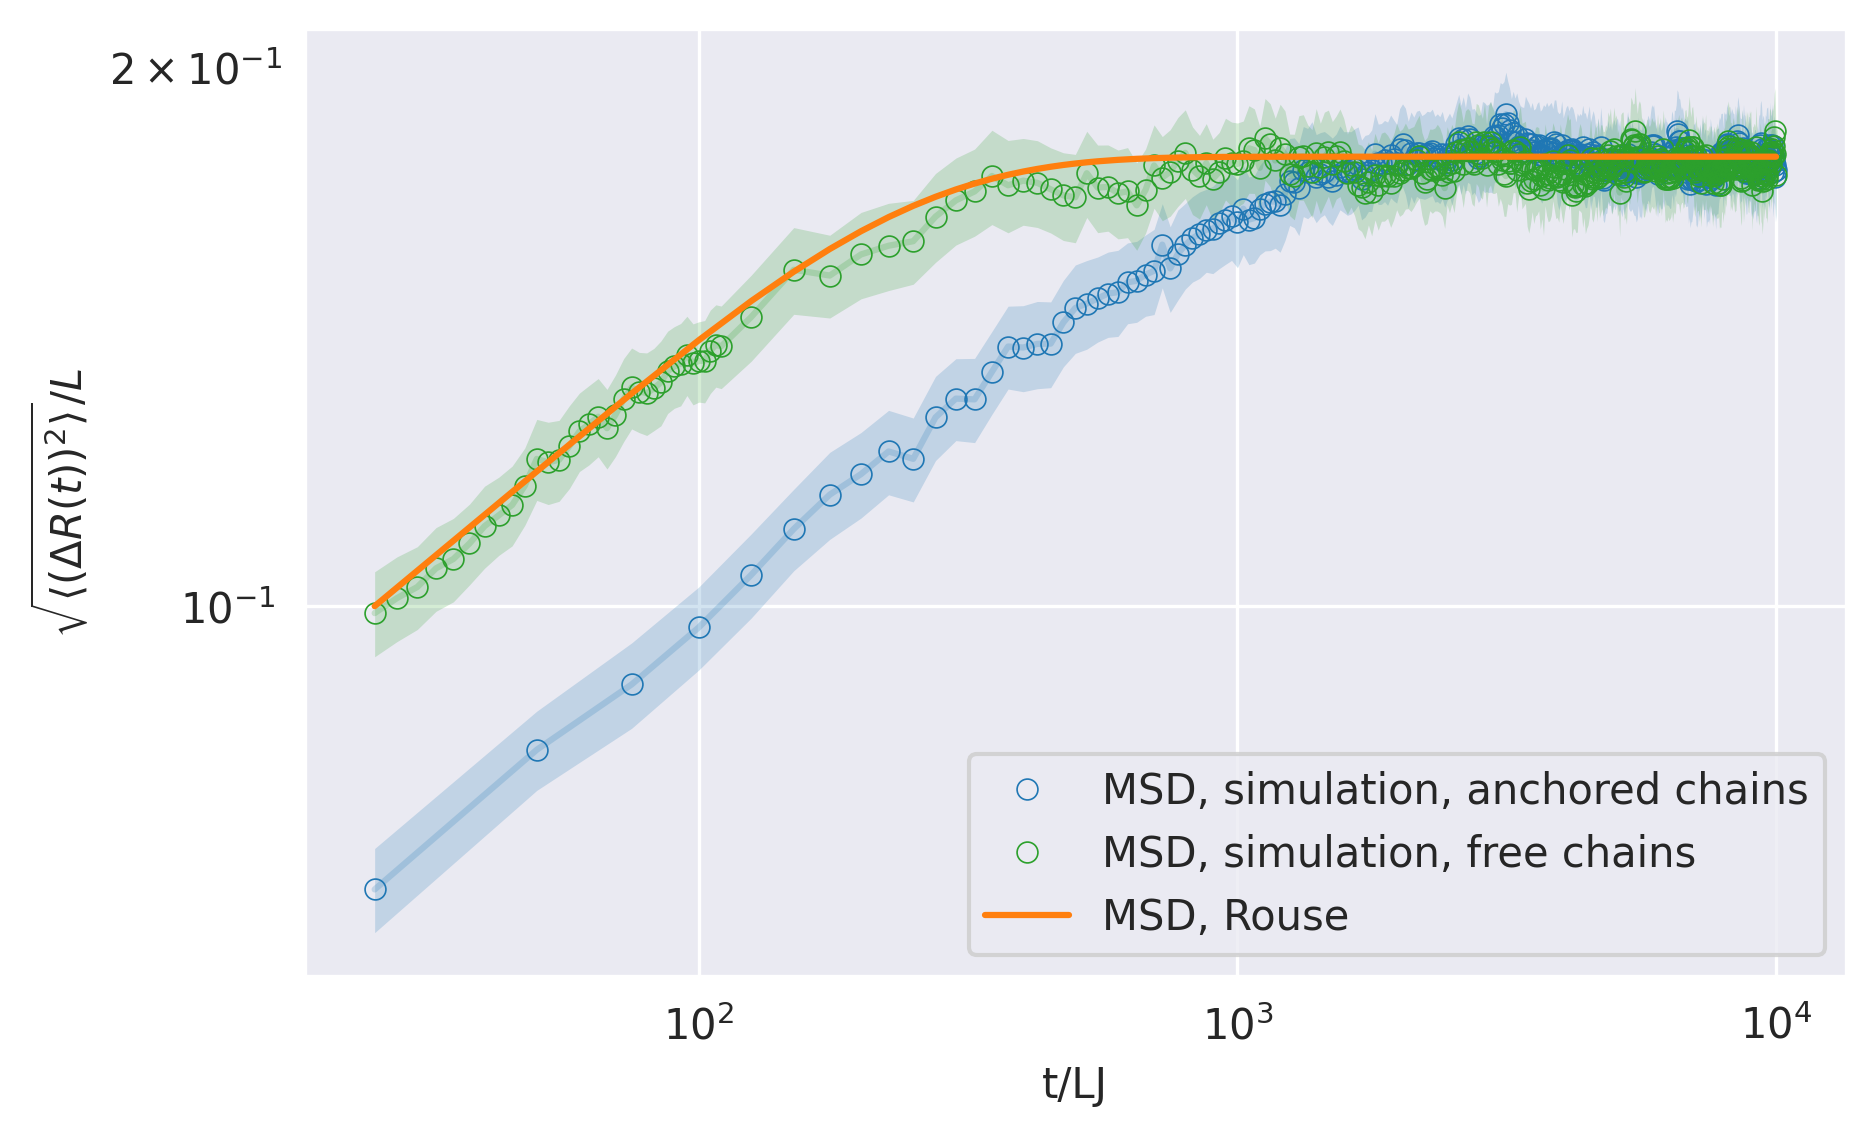
\includegraphics[width=\columnwidth,trim={0cm 0cm 0cm 0.9cm},clip]{3-exp-fixed-param-log.png}
      \caption{\label{fig:anchored_flex_chain_vs_rouse}
      MSD of ETE of anchored full-flexible chain vs predictions of rouse model (free chain, Eq. \ref{eq:rouse_msd_ete}).
      Filled area corresponds MSD curve $\pm$ 3 standard deviations of the mean. The
      line connecting data points and the filled area between data points doesn't make
      any statements about probability of measuring values in this interval and is
      added for readability.
      }
    \end{center}
\end{figure}

\autoref{fig:anchored_flex_chain_vs_rouse} shows, that by anchoring the chain
the transition into plateau is shifted to the right, increasing the 
relaxation time (Eq. \ref{eq:rouse_relaxation_time}), 
however the scaling behavior is visually the same. Rouse relaxation time
of the free chain predicted using rouse model is: $\tau_R=130.16$, $\tau_0=0.941$. 
The rouse relaxation time of the anchored chain estimated 
using the fit of the Eq. \ref{eq:rouse_msd_ete} with $\tau_R$ as free parameter
to the MSD curve of acnhored chain is: 
$\tau_R=582.3 \pm 28.6$, $\tau_0=4.21 \pm 0.07$, which is approximately $4.47$ times
larger. The fitted curve is displayed on
\autoref{fig:anchored_flex_chain_vs_rouse_fitted}.
Intuitively such difference is clear, the beginning of the anchored chain
can't move and therefore the chain needs more time to achieve the MSD limit, which
in case of fully flexible free chain is $2Nl_b^2$ as the one can see from Eq. \ref{eq:rouse_msd_ete}. 


\begin{figure}
    \begin{center}
      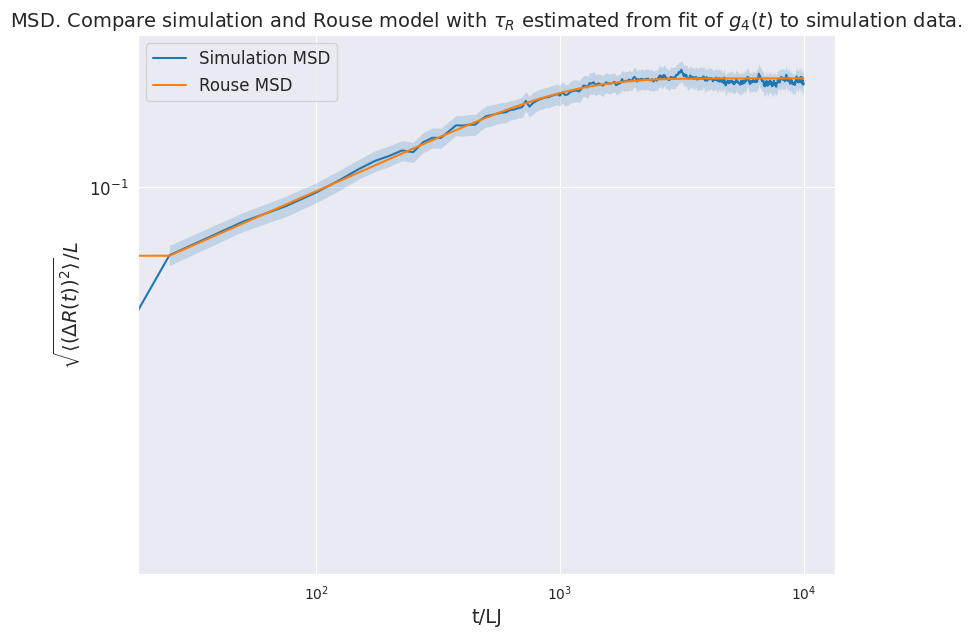
\includegraphics[width=\columnwidth,trim={0cm 0cm 0cm 0.8cm},clip]{3-exp-free-param-log.png}
      \caption{\label{fig:anchored_flex_chain_vs_rouse_fitted}
      MSD of ETE of anchored full-flexible chain vs fit of rouse model prediction 
      (Eq. \ref{eq:rouse_msd_ete}) with $\tau_R$ as free parameter.
      Filled area corresponds MSD curve $\pm$ 3 standard deviations of the mean. The
      blue line connecting data points and the filled area between data points doesn't make
      any statements about probability of measuring values in this interval and is
      added for readability.
      }
    \end{center}
\end{figure}

It is possible to introduce correction factor based on the estimated $\tau_R$
to account for boundary conditions:
\begin{equation}
    \label{eq:adj_factor_beta}
    \beta := \frac{\tau_{0, \textrm{empirical}}}{\tau_{0, \textrm{analytical}}} \approx 4.47
\end{equation}

\FloatBarrier


\subsubsection{Impact of chain stiffness} \label{sec:impact_of_chain_stiffness}
Within this subsection, the focus shifts 
toward exploring the influence of chain stiffness on
the dynamics of anchored chains. 
By manipulating with angle potential the MSD curves for different values
of Kuhn length $l_K$ were measured. 
The analysis provides insights into 
how varying the chain stiffness exert an influence on the 
dynamics exhibited by anchored chain.
\autoref{table:kappa_values} shows the range of stiffness values examined
in this experiment.
\\
\\
The MSD curves are plotted in \autoref{fig:msd_anchored_l_K} and logarithmic
representation one can find in \autoref{fig:msd_anchored_l_K_log}.
The following observations are made:
\begin{itemize}
    \item The relaxation time grows non-linearly with rising $l_K$
    \item Long time MSD limit grows non-linearly with rising $l_K$,
    however for $l_K/L >= 0.65$ it is not possible to distinguish 
    the curves any more because of the uncertainty.
\end{itemize}

\begin{figure}
    \centering
    \begin{subfigure}[b]{\textwidth}
        \centering
        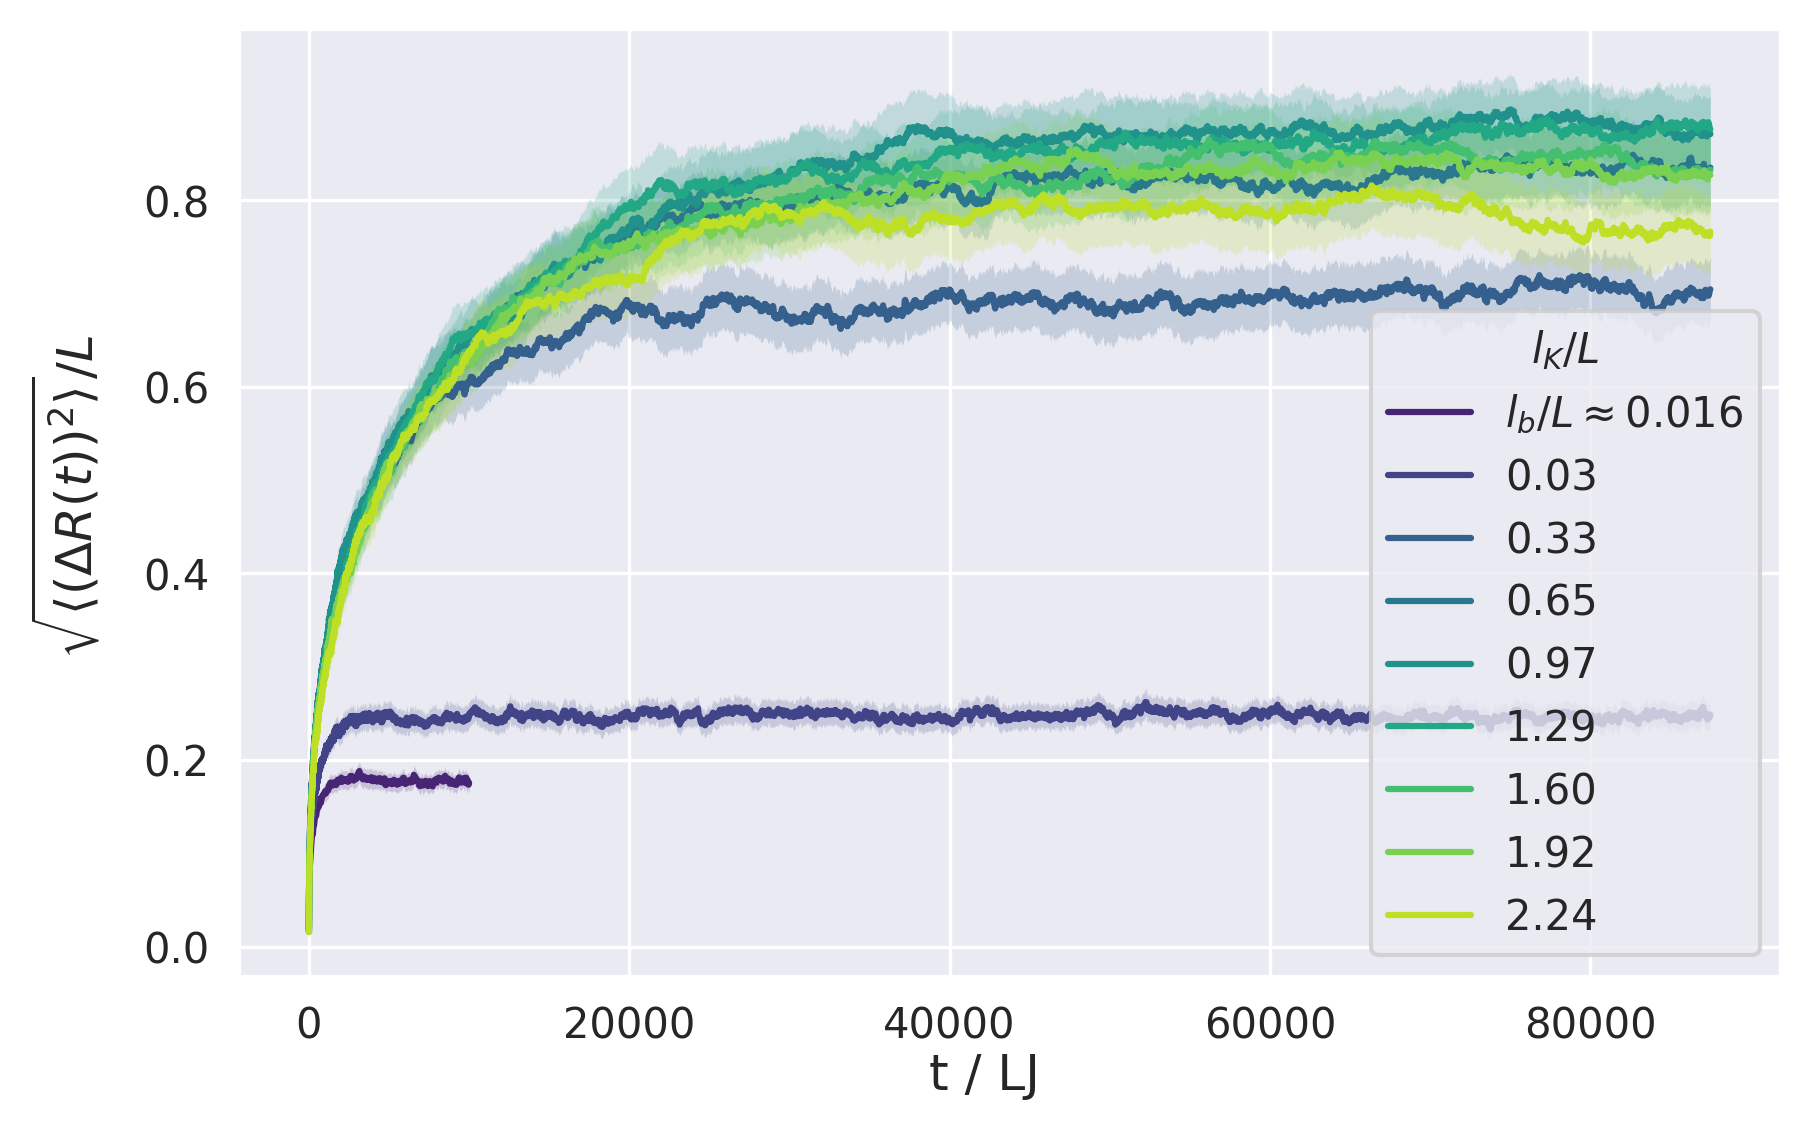
\includegraphics[width=\columnwidth,trim={0cm 0cm 0cm 0.0cm},clip]{4-exp-delta_R-bare.png}
        \caption{\label{fig:msd_anchored_l_K_normal}
        normal scale
        }
    \end{subfigure}
    \begin{subfigure}[b]{\textwidth}
        \centering
        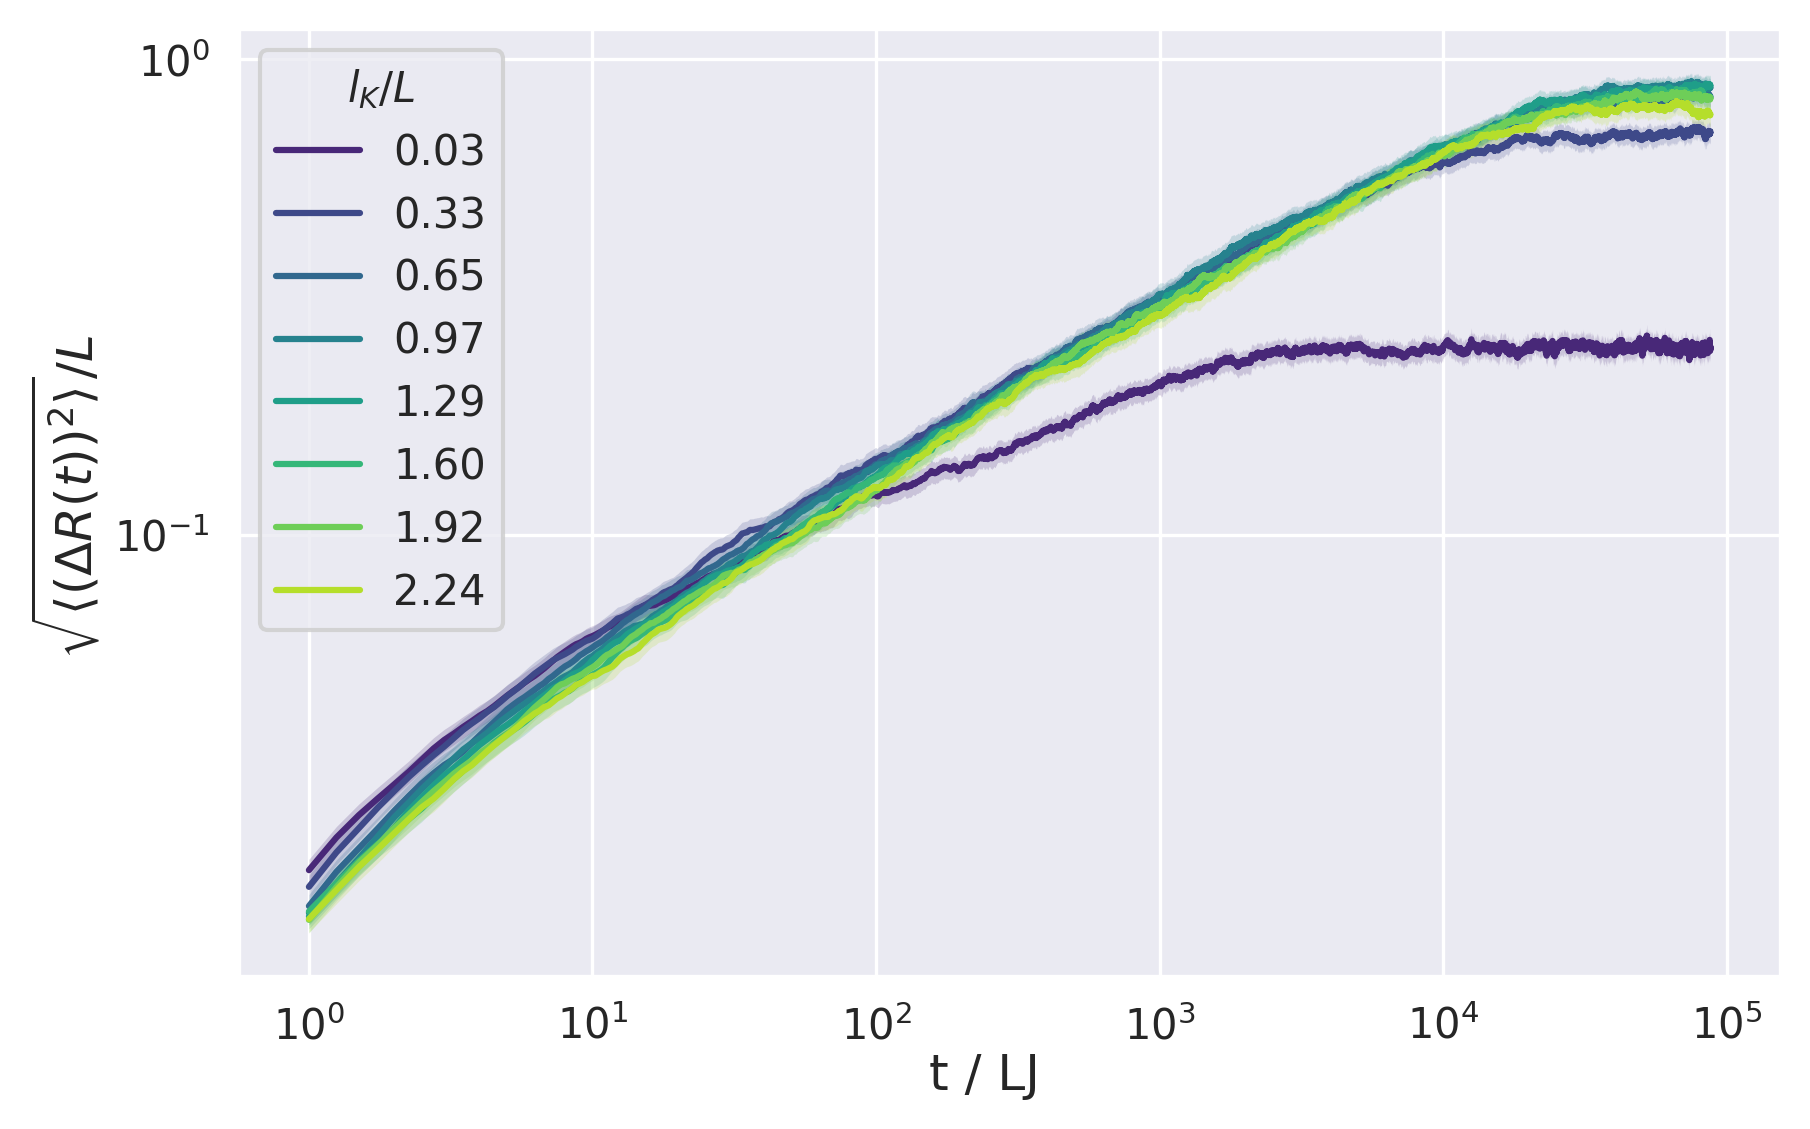
\includegraphics[width=\columnwidth,trim={0cm 0cm 0cm 0.0cm},clip]{4-exp-delta_R-bare-log.png}
        \caption{\label{fig:msd_anchored_l_K_log}
        log scale
        }
    \end{subfigure}
    \caption{Empirical MSD of ETE of anchored chains with different Kuhn length values.
    Filled area corresponds MSD curve $\pm$ 3 standard deviations of the mean.}
    \label{fig:msd_anchored_l_K}
\end{figure}

\begin{table}
    
    \centering
\begin{tabular}{rr}
    \toprule
    $\kappa$ & $l_K / L$ \\
    \midrule
    1.00 & 0.03 \\
    11.00 & 0.33 \\
    21.00 & 0.65 \\
    31.00 & 0.97 \\
    41.00 & 1.29 \\
    51.00 & 1.60 \\
    61.00 & 1.92 \\
    71.00 & 2.24 \\
    \bottomrule
    \end{tabular}
    \caption{
        Values of $\kappa$ and corresponding $l_K$ tried in the study
        of anchored chain dynamics.
        }
    \label{table:kappa_values}
\end{table}

\FloatBarrier

\paragraph{Comparing with Rouse model predictions for flexible chains}

Further, the empirical results are compared to the predictions of the Rouse model.
Firstly, the empirical results are compared to the Rouse model predictions for the fully
flexible chain with $N_K$ segments of length $l_K$. The results of this comparison are shown
in \autoref{fig:msd_anchored_l_K_rouse_fit_anal}. Then the empirical 
results are compared to the Rouse model predictions for fully flexible chain 
with $\tau_R$ as free parameter. The results of this comparison
are displayed in \autoref{fig:msd_anchored_l_K_rouse_fit-tau}. It is clear, 
that Rouse model predictions for fully-flexible chain doesn't match
the observed behavior of semi-flexible anchored chains even with $\tau_R$ as 
free parameter. There are af few possible reasons for that: 
\begin{enumerate}
    \item Violation of contunious chain assumption, because the small number of 
    chain segments
    \item Change of boundary conditions (anchoring).
\end{enumerate}

\begin{figure}
    \begin{center}
      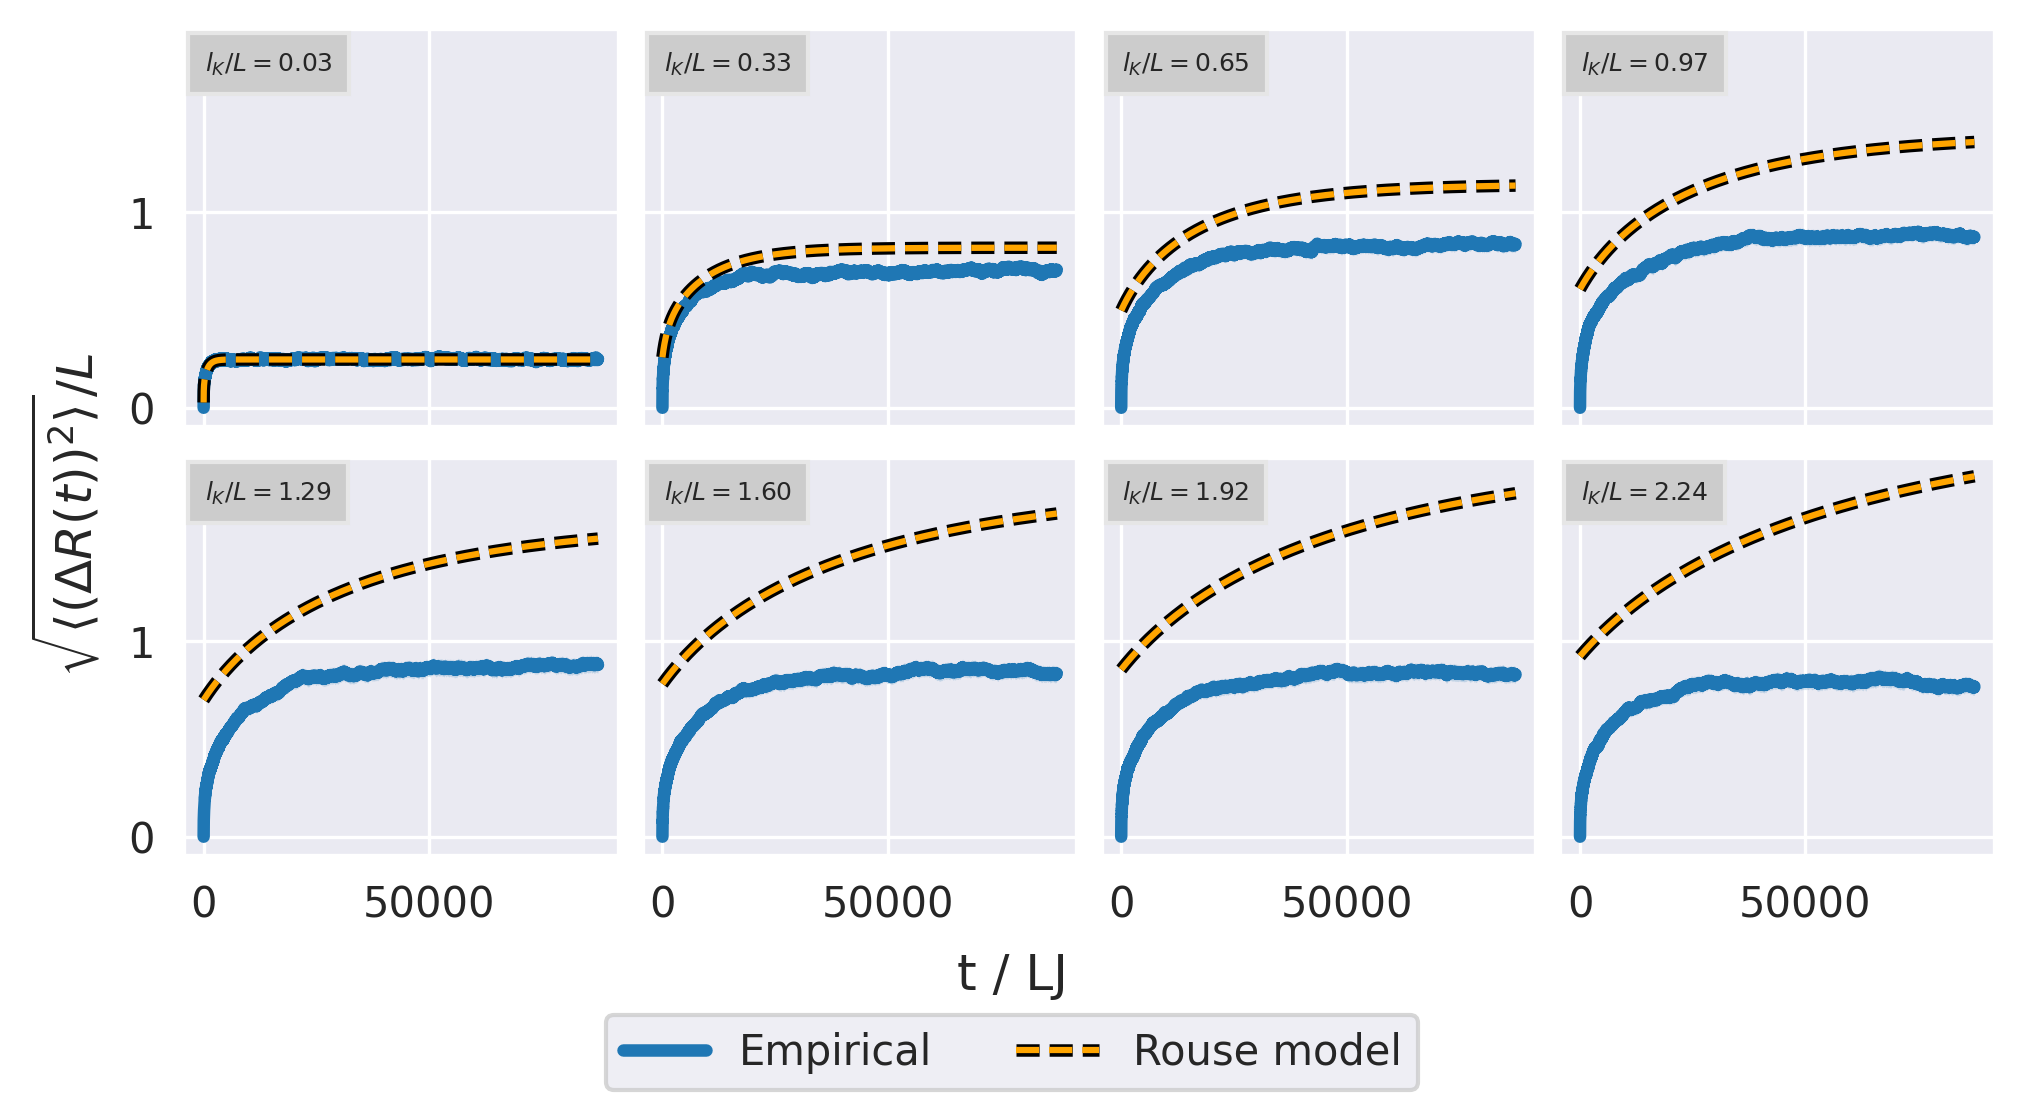
\includegraphics[width=\columnwidth,trim={0cm 0cm 0cm 0.0cm},clip]{4-exp-delta_R-rouse_anal.png}
      \caption{\label{fig:msd_anchored_l_K_rouse_fit_anal}
      Empirical MSD of ETE of anchored chains with different Kuhn length values
      and Rouse model prediction for fully-flexible chains (Eq.\ref{eq:rouse_msd_ete})
      with $N_b = N_K$ if $N_K \ge 1$ or $N_b=1$ otherwise. $\tau_R$ adjusted
      using $\beta$ (Eq.\ref{eq:adj_factor_beta}) to account for boundary conditions.
      }
    \end{center}
\end{figure}
\begin{figure}
    \begin{center}
      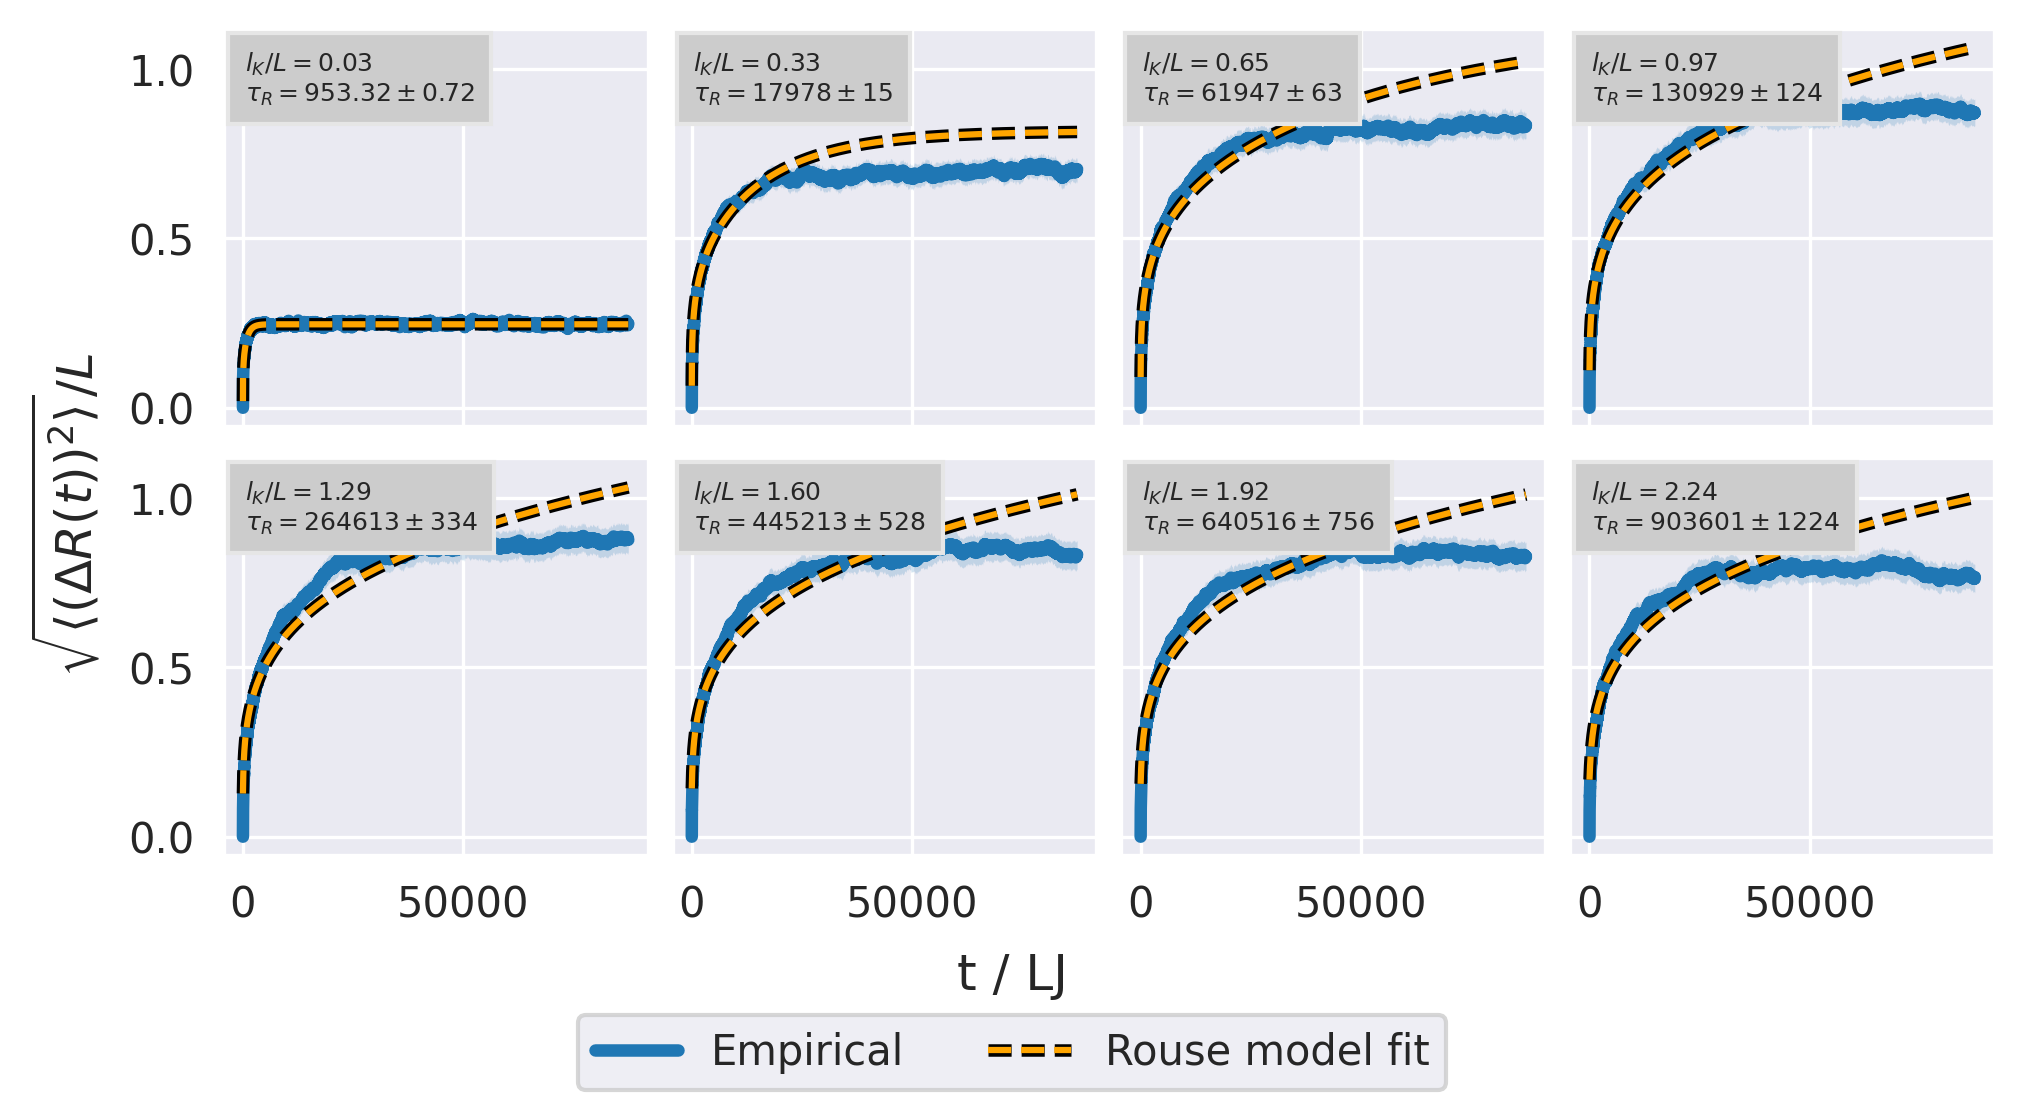
\includegraphics[width=\columnwidth,trim={0cm 0cm 0cm 0.0cm},clip]{4-exp-delta_R-rouse_fit-tau.png}
      \caption{\label{fig:msd_anchored_l_K_rouse_fit-tau}
      Empirical MSD of ETE of anchored chains with different Kuhn length values
      and fit of Rouse model prediction for fully-flexible chains 
      (Eq.\ref{eq:rouse_msd_ete}) with $N_b = N_K$ if $N_K \ge 1$ or $N_b=1$ otherwise.
      $\tau_R$ is free parameter. The summation in Eq.\ref{eq:rouse_msd_ete}
      goes not up to $N_K$ as it strictyly must, but up to number of bonds (63)
      of fully flexible chain.
      }
    \end{center}
\end{figure}

\FloatBarrier

\paragraph{Comparing with Rouse model predictions for semiflexible chains}

Furthermore, the empirical MSD curves are compared to the predictions
of the Rouse model for the semiflexible chains. The autocorrelation function
of End-to-End vector was already discussed in Section \ref{sec:rouse_semiflex_chain}.
The MSD can be written as 
$$\E{[\Delta \vec{R}(t)]^2} = \E{R^2(t)} - 2 \E{\vec{R}(t)\vec{R}(0)} + \E{R^2(0)} = 2(\E{R^2} - \E{\vec{R}(t)\vec{R}(0)})$$
where the term $\E{\vec{R}(t)\vec{R}(0)}$ in case of free semiflexible chain obeys 
the relationships discussed in Section \ref{sec:rouse_semiflex_chain}.

To compare the long time case with empirical results the expression
$2(\E{R^2} - k \exp(-t/\tau_{rot}))$ with $k$ as free paramater was fit 
to the part of corresponding empirical MSD curves as specified in 
Eq. \ref{eq:autocorr_ete_coil_limit_long_time} and Eq. \ref{eq:autocorr_ete_rod_limit}.
The result was then visually examined against empirical curve.
This comparison revealed, that MSD in long time limit based on 
Eq. \ref{eq:autocorr_ete_coil_limit_long_time} and 
Eq. \ref{eq:autocorr_ete_rod_limit} does not correspond to empirical curves.
However, introduction of two meaningfull free parameters ($a$, $\tau_{rot}$) is able to dismiss
the discrepancy between theoretical approach for free chain and empirical 
results for anchored chain:
\begin{equation}
    \label{eq:adjusted_rouse_model_ete}
    \E{[\Delta \vec{R}(t)]^2}  = a\E{R^2}[1 - exp(-\frac{t}{\tau_{rot}})]
\end{equation}
The free parameter $a$ accounts for large-time limit of MSD and $\tau_{rot}$ 
accounts location of the transition into the plateau. However, one
can only speculate, that new $\tau_{rot}$ has the same meaning
as the old one. The results of this fit are shown in 
\autoref{fig:msd_anchored_l_K_rouse_fit_tau-a}.
It is possible to conclude, that in case of anchored chain the proportionality
$\E{\vec{R}(t)\vec{R}(0)} \propto exp(-\frac{t}{\tau_{rot}})$
holds for $t>\tau_{rot}$ but with different value (and eventually meaning) of $\tau_{rot}$.
In case of the chains close to rod-limit the one can see that in analogy with 
the case of free chains in rod limit there should be some analogy of 
characteristic time $\tau_1$ (from Eq. \ref{eq:autocorr_ete_rod_limit}) which 
is smaller then estimated $\tau_{rot}$ and where the above mentioned 
proportionality starts to be valid.

\begin{figure}
    \centering
    \begin{subfigure}[b]{\textwidth}
        \centering
        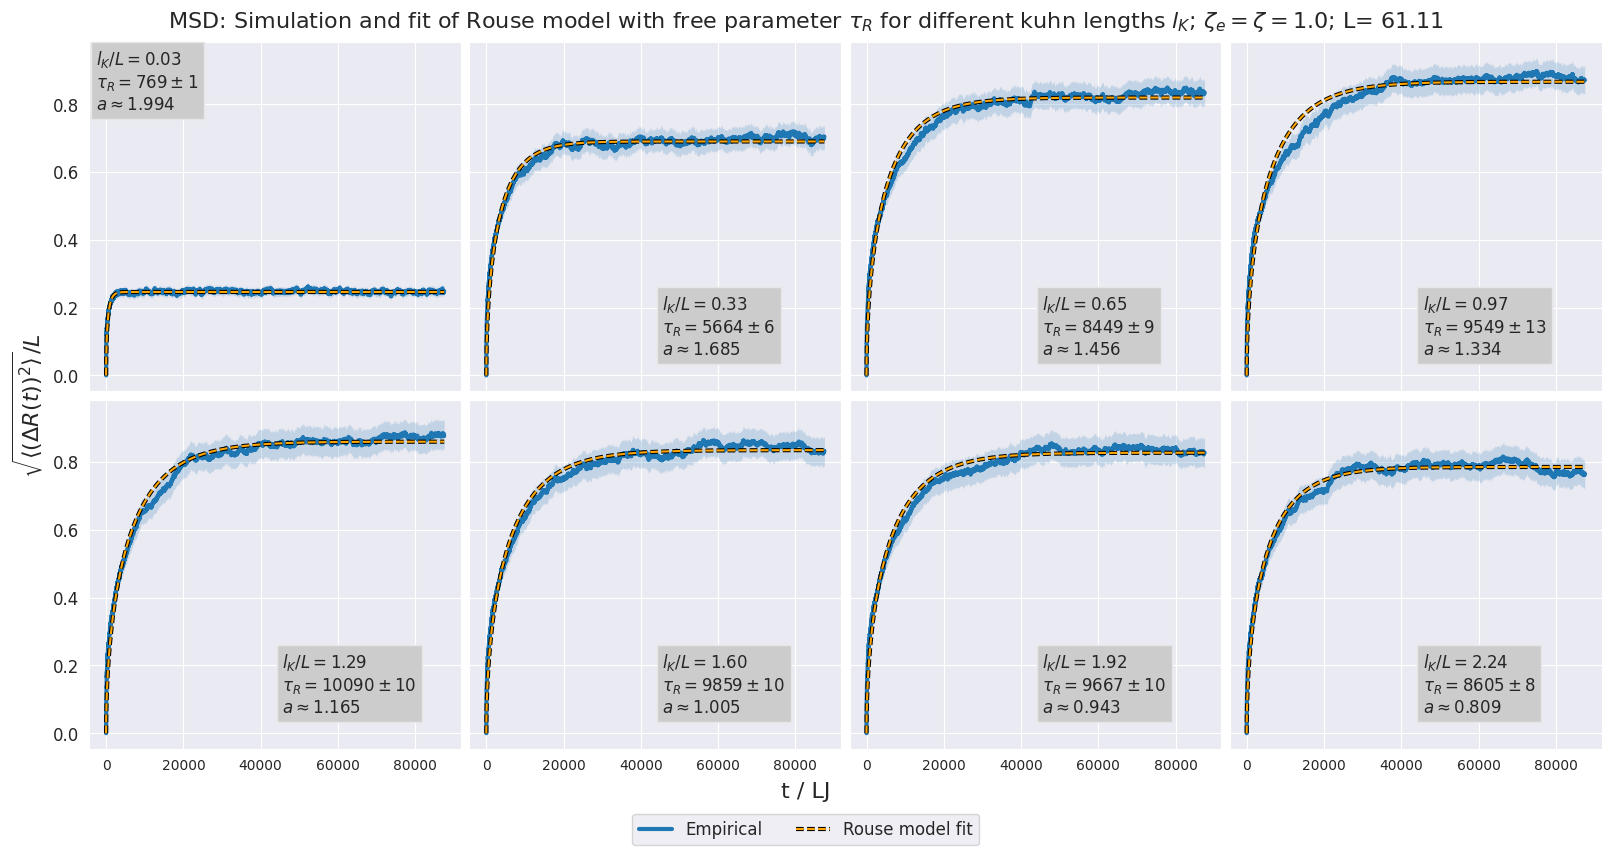
\includegraphics[width=\textwidth]{4-exp-delta_R-rouse_fit-tau-a.png}
        \caption{normal scale}
        \label{fig:msd_anchored_l_K_rouse_fit_tau-a_normal}
    \end{subfigure}
    \begin{subfigure}[b]{\textwidth}
        \centering
        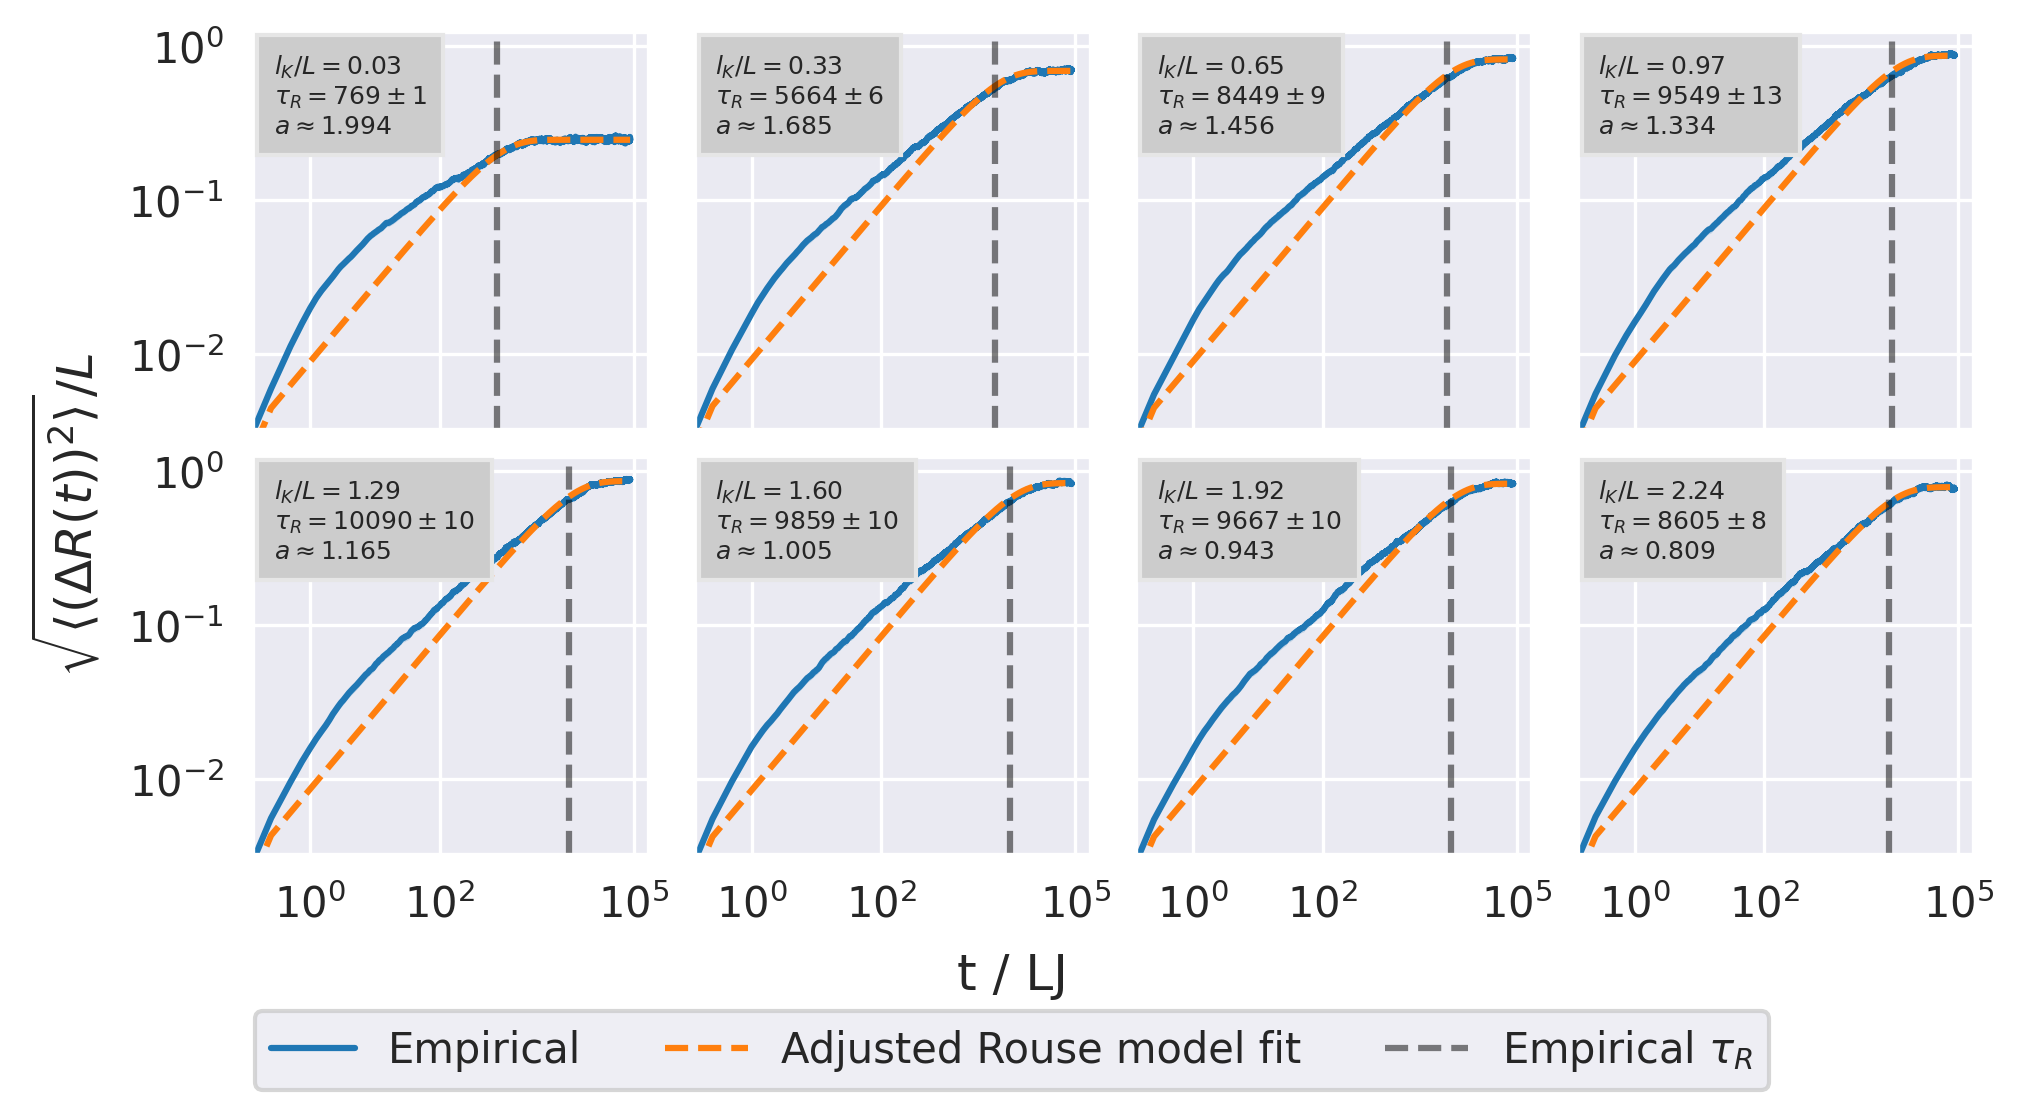
\includegraphics[width=\textwidth]{4-exp-delta_R-rouse_fit-tau-a_log.png}
        \caption{log-log scale}
        \label{fig:msd_anchored_l_K_rouse_fit_tau-a_log}
    \end{subfigure}
    \caption{Empirical MSD of ETE of anchored chains with different Kuhn length values (blue line)
    and fit of modified Rouse model prediction for semi-flexible chains 
    (Eq.\ref{eq:adjusted_rouse_model_ete}, dashed line) on log-log scale.
    Estimated (empirical) $\tau_{rot}$ is drawn as vertical dashed line.}
    \label{fig:msd_anchored_l_K_rouse_fit_tau-a}
\end{figure}

\vspace{0.5cm}
Further, the case of short times is examined. To execute this comparison
the scaling behavior of empirical MSD is analyzed. It is clear, that
$\E{[\Delta \vec{R}(t)]^2} \propto t^{\alpha(t)}$ for the small times is valid
in analogy to scaling behavior of MSD of last monomer of free chain. 
The scaling exponent $\alpha$ is estimated from MSD curves as 
described in Section \ref{sec:est-alpha-msd} with $n=10$ bins. 
The result is shown on \autoref{fig:alpha_anchored_l_K}.
Further in this paragraph $\alpha_{min}$ refers to scaling exponent $\alpha$
in region where the overdamped motion takes place and $t \ll \tau_{rot}$. 
For nearly flexible chain $l_K/L = 0.03$ $\alpha_{min} \approx \frac{1}{2}$
is observed, which matches theoretical expectations for fully flexible chain.
For semi-flexible chains the value $\alpha_{min}$ is close to $\frac{3}{4}$, which
matches the scaling behavior of free chain at short times. 
One can see, that $\alpha_{min}$ gets closer to $\frac{3}{4}$ with rising $l_K$. Larger
scaling factor in the region $[1, 10]$ is due to transition from 
ballistic motion at time scales $t<\frac{1}{\sigma} = 1$ to the overdamped motion.
Additionaly, $\alpha$ for $t>\tau_{rot}$ matches the one of rouse model prediction
for free semiflexible chain as well as $\alpha$ transitions in this regime smoothly
near the $\tau_{rot}$.

\begin{figure}[h]
    \begin{center}
      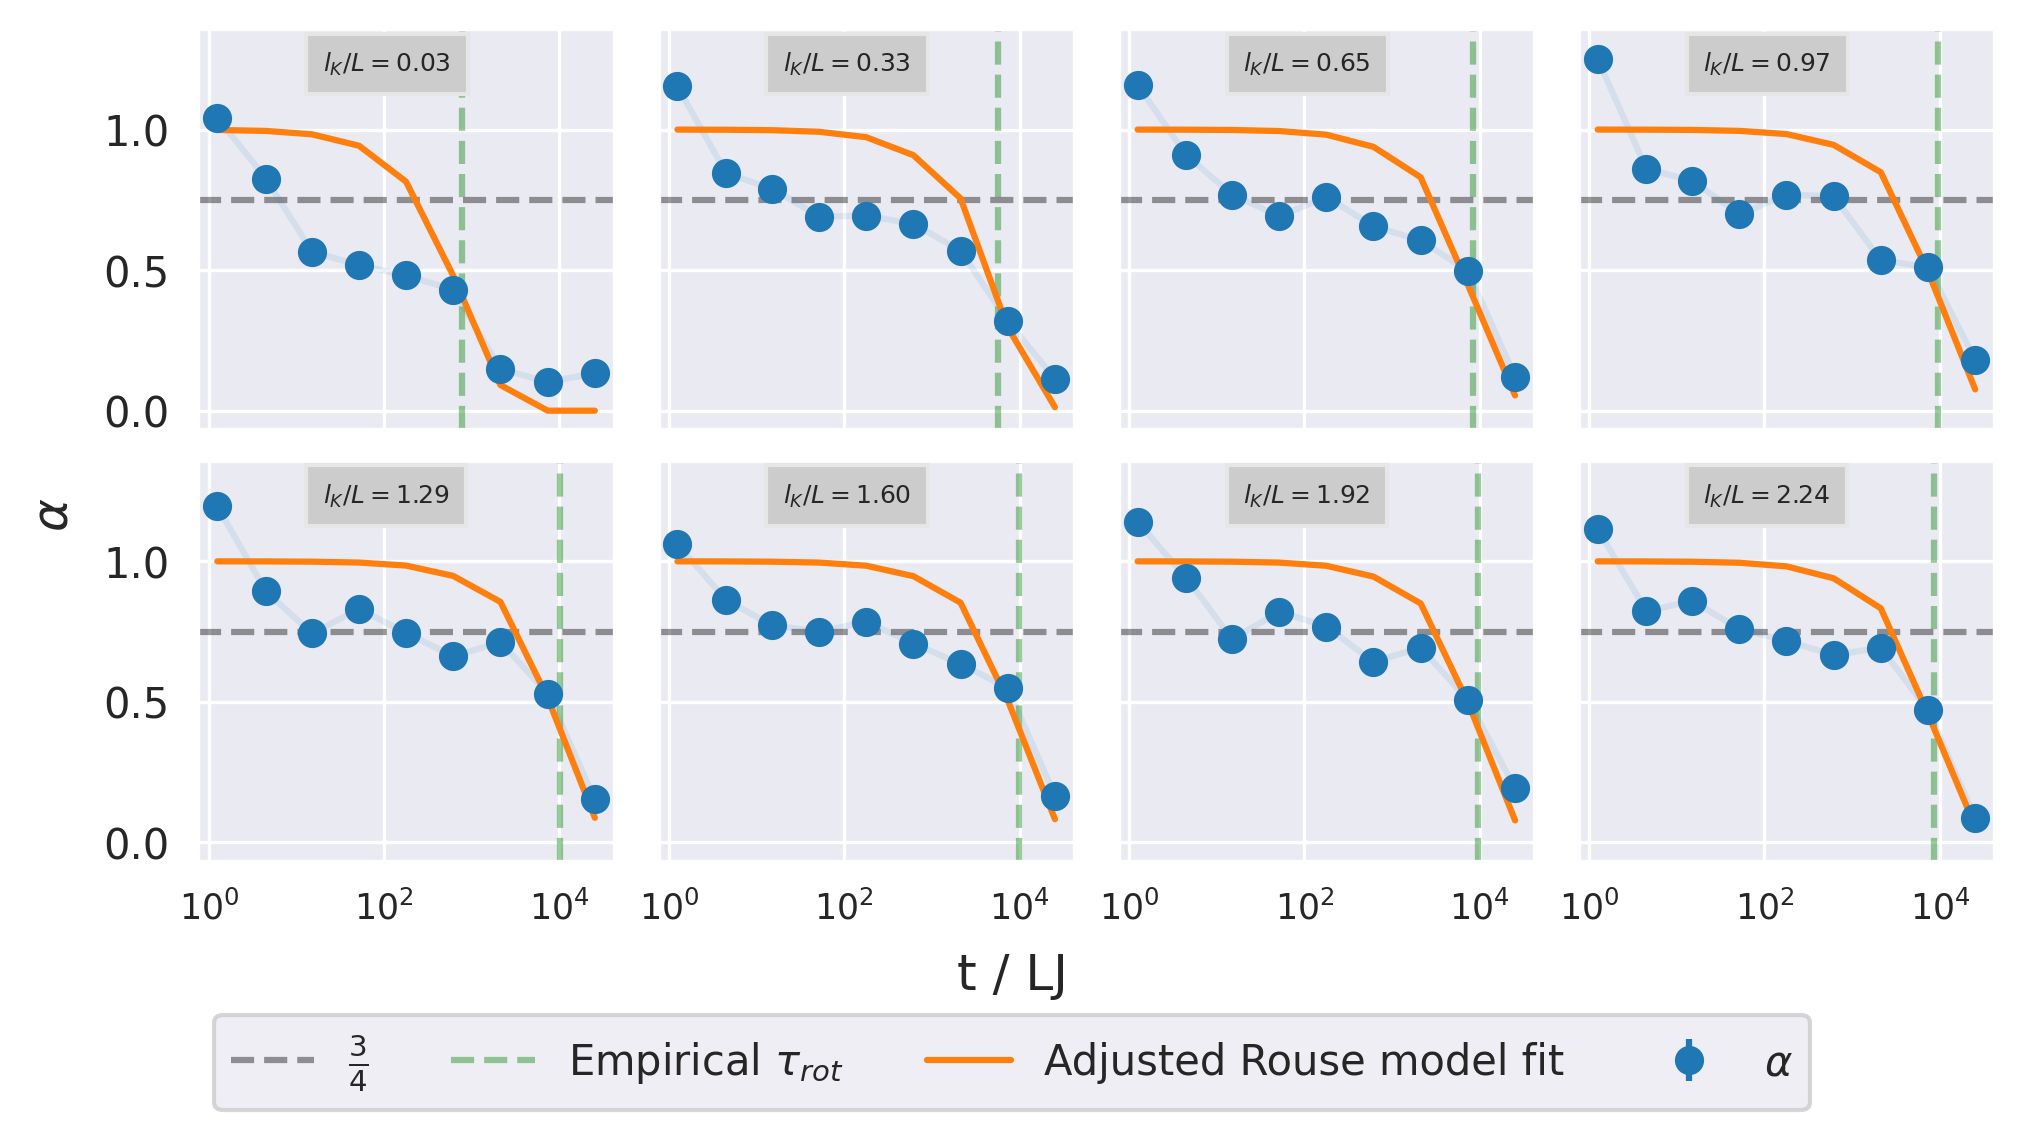
\includegraphics[width=\columnwidth,trim={0cm 0cm 0cm 0.0cm},clip]{4-exp-delta_R-rouse_fit-tau-a_alpha.png}
      \caption{\label{fig:alpha_anchored_l_K}
      Scaling exponent $\alpha$ of the MSD of ETE of anchored semiflexible chain (blue points) and 
      scaling exponent $\alpha$ of modified Rouse model prediction for semi-flexible chains 
      (Eq.\ref{eq:adjusted_rouse_model_ete}, orange line).
      Estimated (empirical) $\tau_{rot}$ is drawn as vertical dashed line.
      Horizontal grey dashed line corresponds to $\frac{3}{4}$ value.
      }
    \end{center}
\end{figure}

\FloatBarrier


\paragraph{Main-axis system perspective}
Further, the MSD in main-axis coordinate system is analyzed.
\autoref{fig:msd_anchored_l_K_by_dim} shows the MSD curves in main axis system
for each dimension. The analysis delivers following insights:
\begin{itemize}
    \item The difference of MSD in $z$ dimension relative to the $x$ and $y$
    dimensions rises with growing stiffness. The plateau value of MSD falls.
    \item The MSD in $z$ dimension has smaller relaxation time in case $l_K/L \ge 0.95$ 
\end{itemize}
The chain becomes more straight with rising stiffness and therefore has less
movement freedom along $z$ direction, which results in smaller MSD and quicker
relaxation.

\begin{figure}
    \begin{center}
      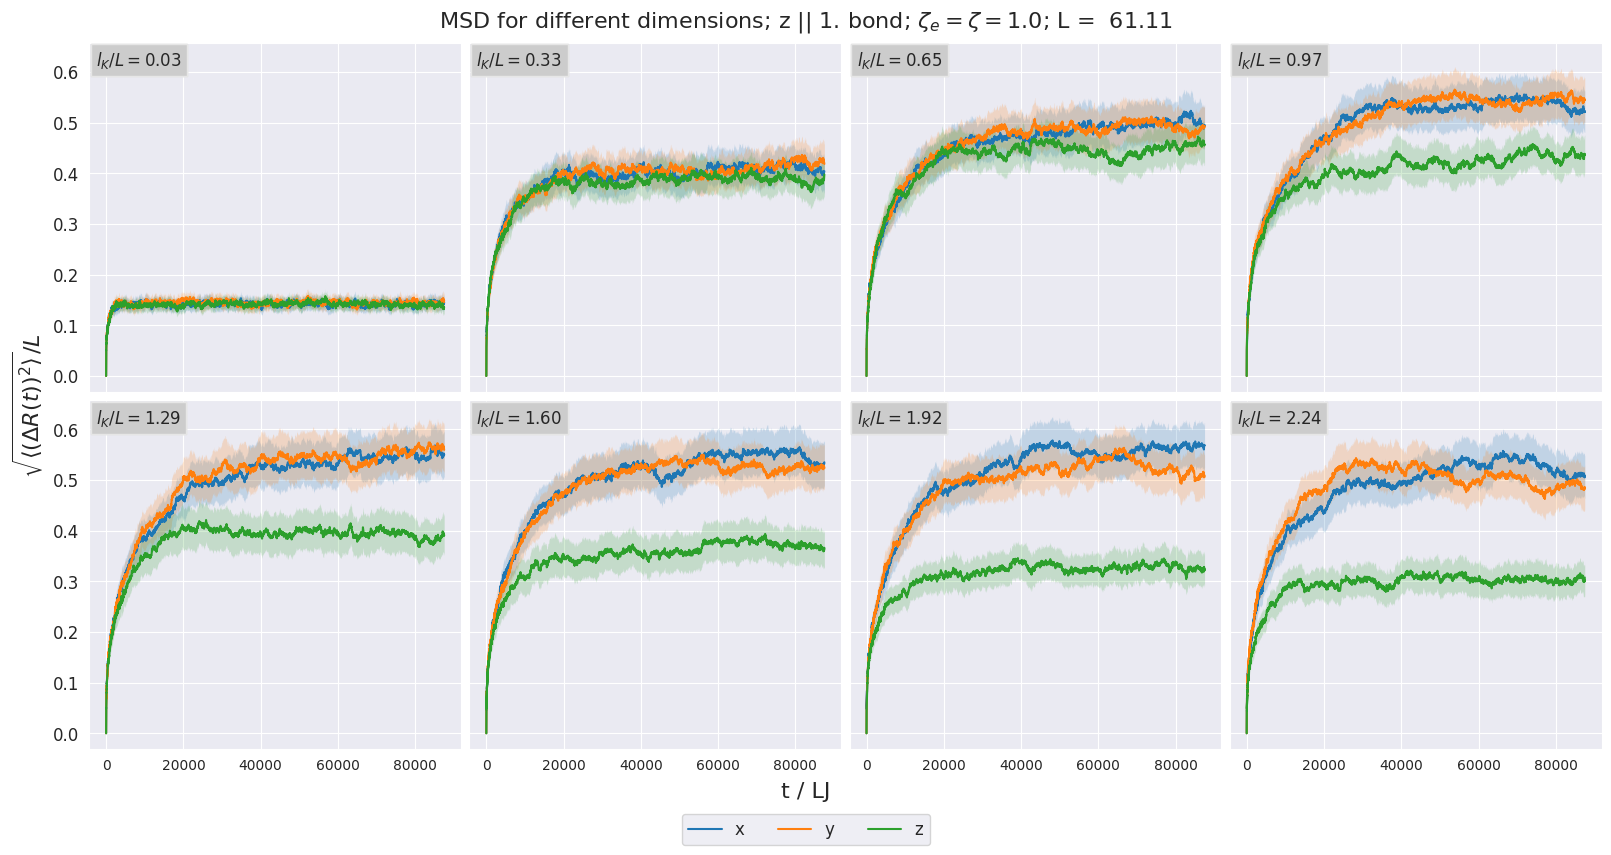
\includegraphics[width=\columnwidth,trim={0cm 0cm 0cm 0.0cm},clip]{4-exp-msd_by_dim.png}
      \caption{\label{fig:msd_anchored_l_K_by_dim}
      Empirical MSD of ETE of anchored chains with different Kuhn length values in
      main-axis coordinate system (See section \ref{sec:main-axis}).
      }
    \end{center}
\end{figure}

\FloatBarrier

\subsubsection{Impact of friction coefficient of chain end}
In this subsection, the focus turns to the influence 
of the friction coefficient at the chain end on the dynamics of anchored chain with high
stiffness.
\\
\\
In the simulation this is achieved by changing the value of damp parameter of Langevin thermostat
for the last bead of the chain. Assuming the Stokes friction, 
changing the value of damp parameter effectively means change of the mass or change of the 
bead diameter. The mass of the end bead is set to the $m_e = 1.5$ and friction coefficient of end bead
is varied: $\zeta_e = 10, 15$, which corresponds to the end-bead diamaters: $15, 30$.
The reference value provides simulation of the chain with $\zeta_e=\zeta=1$ and $m_e=m=1$.
In all 3 cases $\kappa=190.2$, which results in Kuhn length $l_K/L=6.02$. The chosen
persistence length of the chains relative to their contour length $l_p/L=l_K/(2L)=3.01$ matches
the one of the unbound EEA1 \cite{Singh:2022}.

\paragraph{Comparing with Rouse model}
The approach mostly follows section \ref{sec:impact_of_chain_stiffness} with an exception that
the friction coefficient of the chain end $\zeta_e$ is varied instead of Kuhn length $l_K$ 
of the chain. The resulting MSD curves are shown on 
\autoref{fig:msd_anchored_zeta}. Again, Adjusted Rouse model 
(Eq. \ref{eq:adjusted_rouse_model_ete}) is fited to
the MSD curves: \autoref{fig:msd_anchored_zeta-arm_fit}. The one can see
the perfect match on time scales $t > \tau_{rot}$. Also, the estimated $\tau_{rot}$
rise with rising $\zeta_e$ and the scaling behavior on short time scales 
varies. To investigate the scaling behavior the scaling exponent $\alpha$ is
calculated as described in Section \ref{sec:est-alpha-msd} 
within $n=20$ bins and is plotted on \autoref{fig:alpha_anchored_zeta}.
The rouse model for semiflexible free chains predicts $\alpha=3/4$ on the
time scales $t < \tau_{1} \ll \tau_{rot}$. To test if this holds for chains with larger
friction coefficient of the chain end it's necessary to estimate $\alpha$ in this
region. The $\alpha_m := \alpha \text{ for } t \ll \tau_{rot}$ is defined.
Based on \emph{Nikoubashman et. al.} \cite{Nikoubashman2016} finding,
that the crossover from ballistic motion to anomalous diffusion, as described 
in Rouse model, lasts 2 decades of time, it is assumed, 
that the left border of this region is given by the end of the region of ballistic
motion of the end bead $\tau_b  := 10 \frac{m}{\zeta_e}$. The right border is
assumed to be $\tau_{rot} / 10$ to match $t \ll \tau_{rot}$ requirement.
The borders of the region are plotted with red dashed line and vizually match
the observed scaling behavior. The $\alpha_m$ is then calculated as the mean
of observed $\alpha$ in the region. The measurement uncertainty is estimated
as 3 standard deviations of the mean. All estimated quantities are summarized
in table \ref{table:anchored_chain_zeta_estimations}. The one can see the 
small increase of $\alpha_m$ by transition from $\zeta_e=1$ to $\zeta_e=10$ and, 
given the confidence interval, there is no difference between 
$\alpha_m$ for $\zeta_e = 10$ and $\zeta_e=20$.

\paragraph{Main-axis system perspective}
Additionaly different dimensions of MSD in main-axis coordinate system are
analyzed and results are shown on \autoref{fig:msd_anchored_zeta-dim}.
The one can observe, that the visual patterns of 
increasing $\zeta_e$ for all dimensions are the same.

\begin{figure}
    \centering
    \begin{subfigure}[b]{\textwidth}
        \centering
        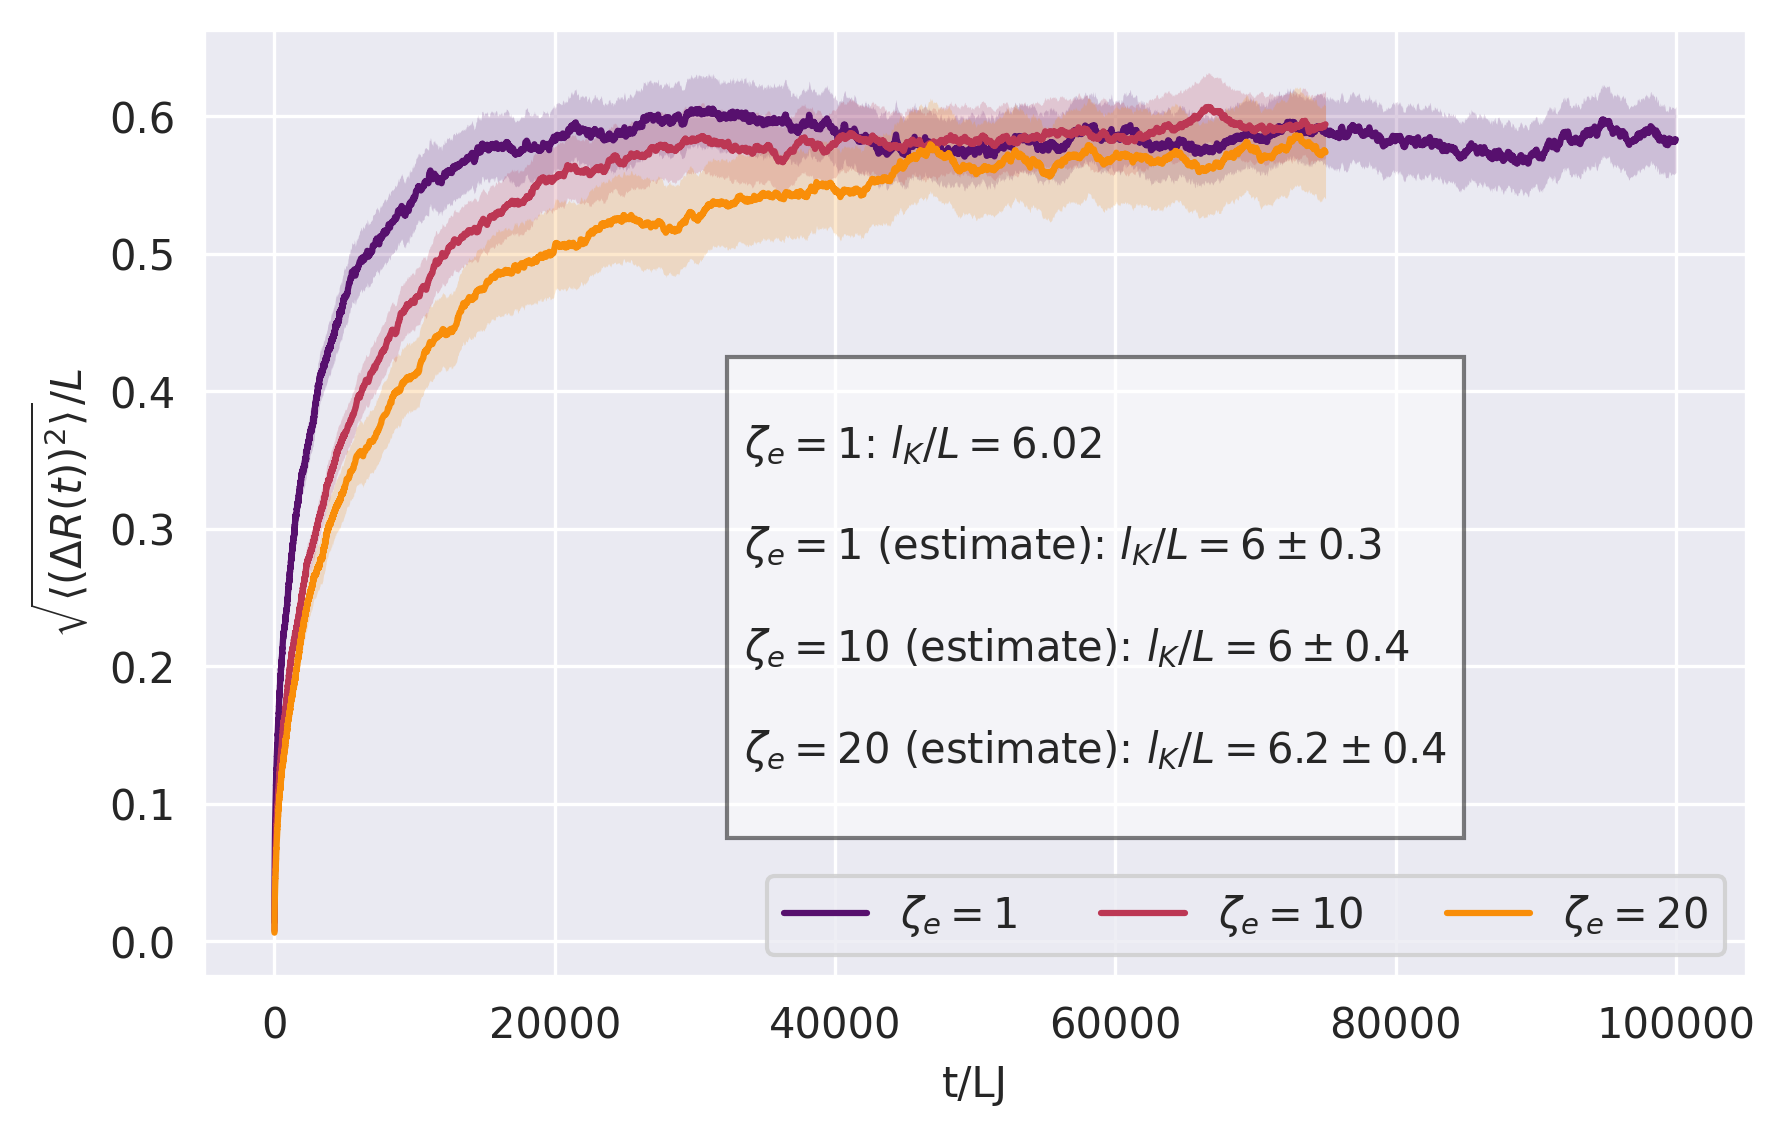
\includegraphics[width=\textwidth]{14+15+16-exp-msd.png}
        \caption{normal scale}
        \label{fig:msd_anchored_zeta-normal}
    \end{subfigure}
    \begin{subfigure}[b]{\textwidth}
        \centering
        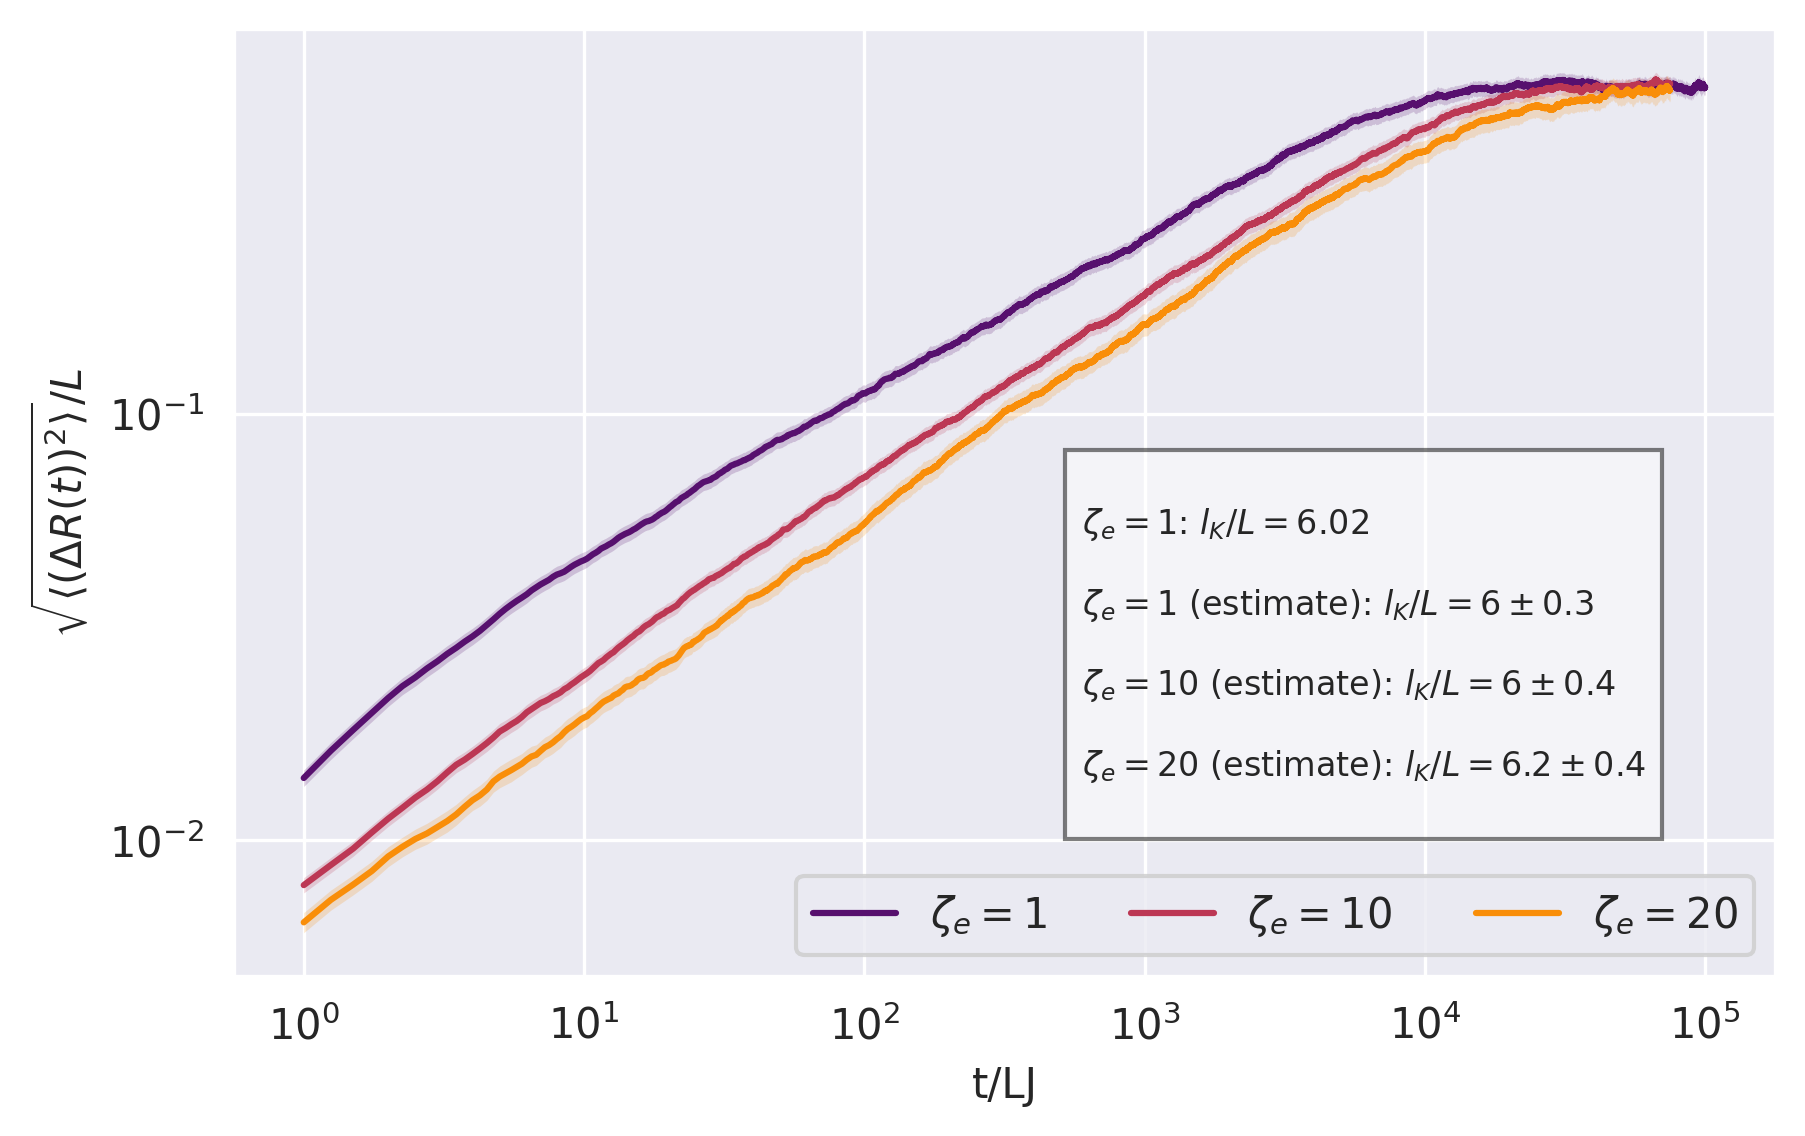
\includegraphics[width=\textwidth]{14+15+16-exp-msd-log.png}
        \caption{log-log scale}
        \label{fig:msd_anchored_zeta-log}
    \end{subfigure}
    \caption{Empirical MSD of ETE of anchored chains with different values of
    friction coefficient of the chain end $\zeta_e$. 
    Configured and estimated Kuhn length is shown in text box (as
    additional check of plausibility).
    Estimation of Kuhn length is done using fit of 
    \autoref{eq:worm-like-chain-cos-theta-ij} with $l_p$ as free parameter.
    }
    \label{fig:msd_anchored_zeta}
\end{figure}

\begin{figure}
    \centering
    \begin{subfigure}[b]{\textwidth}
        \centering
        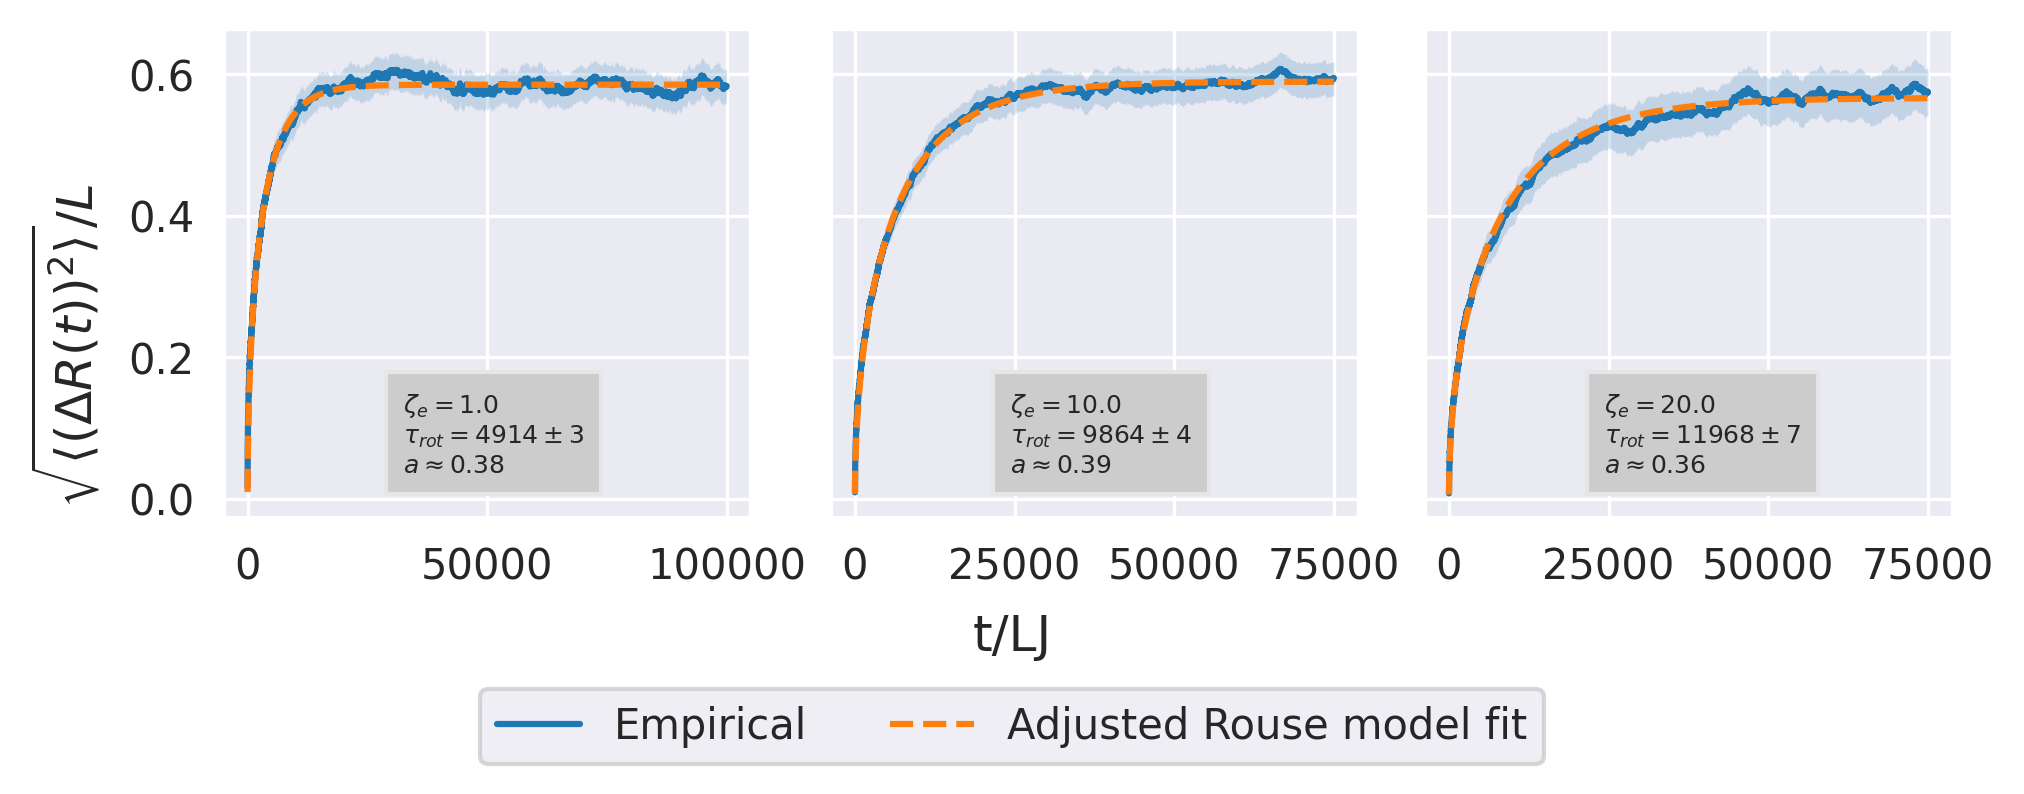
\includegraphics[width=\textwidth]{14+15+16-exp-msd-log-arm_fit.png}
        \caption{normal scale}
        \label{fig:msd_anchored_zeta-arm_fit-normal}
    \end{subfigure}
    \begin{subfigure}[b]{\textwidth}
        \centering
        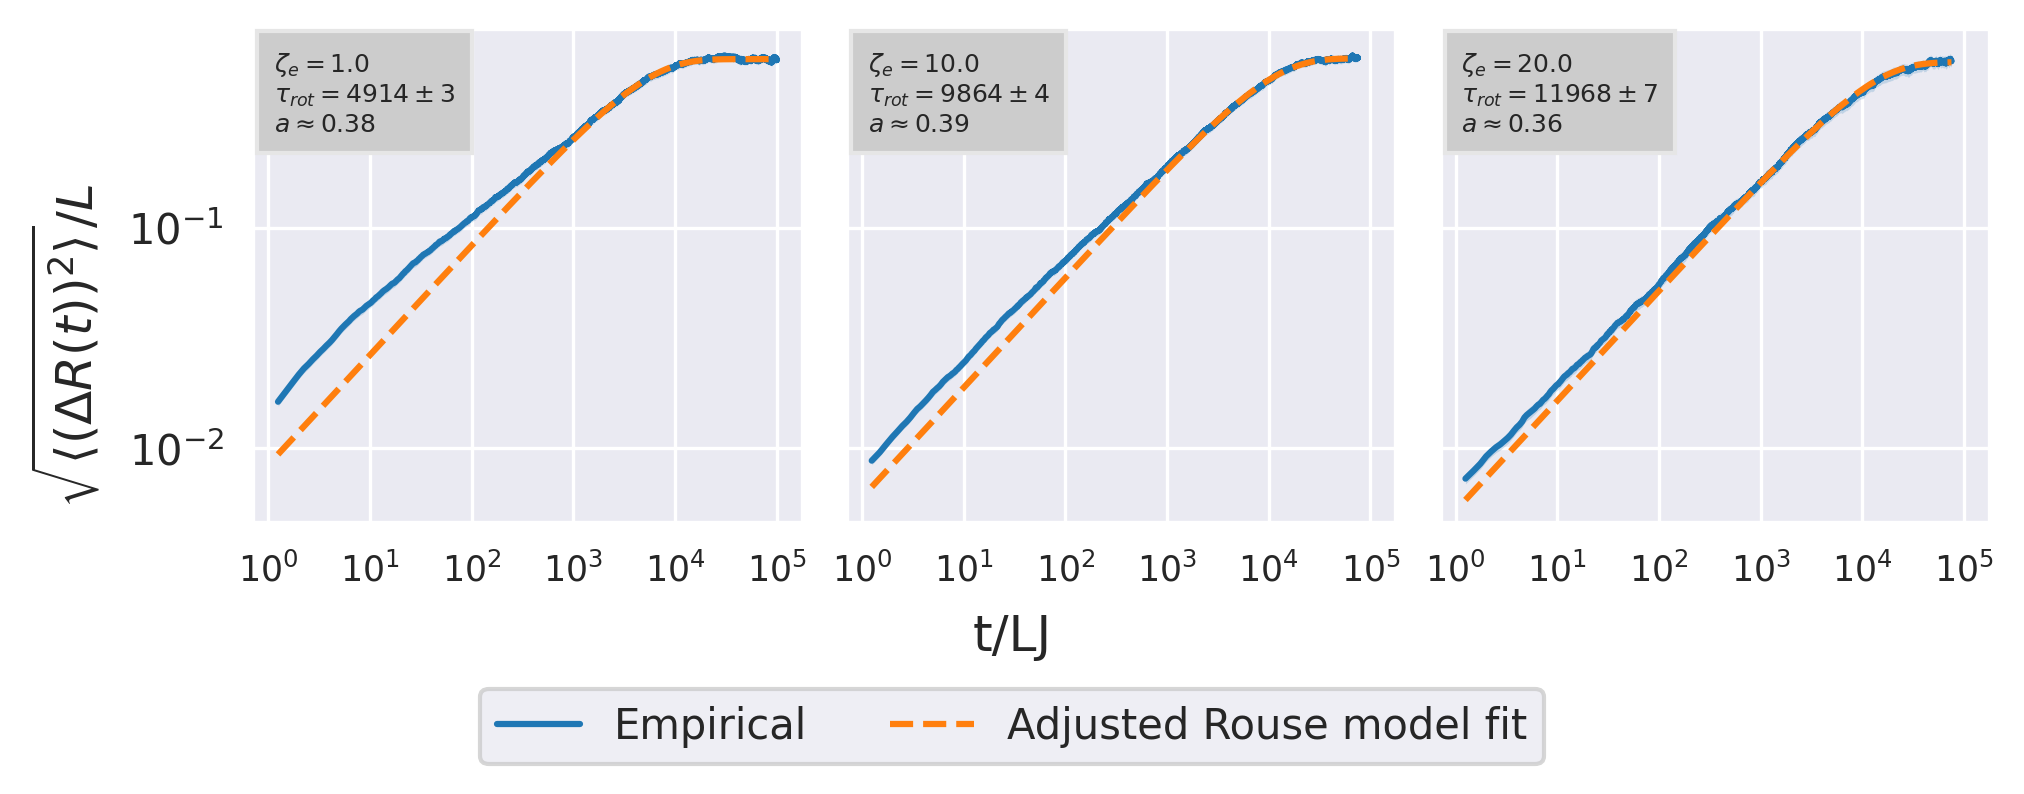
\includegraphics[width=\textwidth]{14+15+16-exp-msd-log-arm_fit-log.png}
        \caption{log-log scale}
        \label{fig:msd_anchored_zeta-arm_fit-log}
    \end{subfigure}
    \caption{Empirical MSD of ETE of anchored chains with different values of
    friction coefficient of the chain end $\zeta_e$ and corresponding fit
    of the Adjusted Rouse model (Eq.\ref{eq:adjusted_rouse_model_ete}).
    }
    \label{fig:msd_anchored_zeta-arm_fit}
\end{figure}

\begin{table}
    \centering
    \begin{tabular}{lrrrrrrr}
        \toprule
         & $\tau_{rot}$ & $\Delta \tau_{rot}$ & $a$ & $\Delta a$ & $m_e$ & $\alpha_m$ & $\Delta \alpha_m $\\
        $\zeta_e$ &  &  &  &  &  &  &  \\
        \midrule
        1 & 4914.250775 & 2.551632 & 0.381353 & 0.000096 & 1.0 & 0.736970 & 0.055872 \\
        10 & 9863.543716 & 3.602848 & 0.387068 & 0.000071 & 1.5 & 0.919990 & 0.067072 \\
        20 & 11967.770149 & 7.068073 & 0.357454 & 0.000103 & 1.5 & 0.928494 & 0.070997 \\
        \bottomrule
    \end{tabular}
    \caption{
        Anchored chain, $l_K/L=6.02$. 
        Estimated values of free parameters of Adjusted Rouse model (Eq.\ref{eq:adjusted_rouse_model_ete}),
        estimated scaling exponent $\alpha_m$ and corresponding $\zeta_e$ and $m_e$ values.
    }
    \label{table:anchored_chain_zeta_estimations}
\end{table}


\begin{figure}
    \centering
    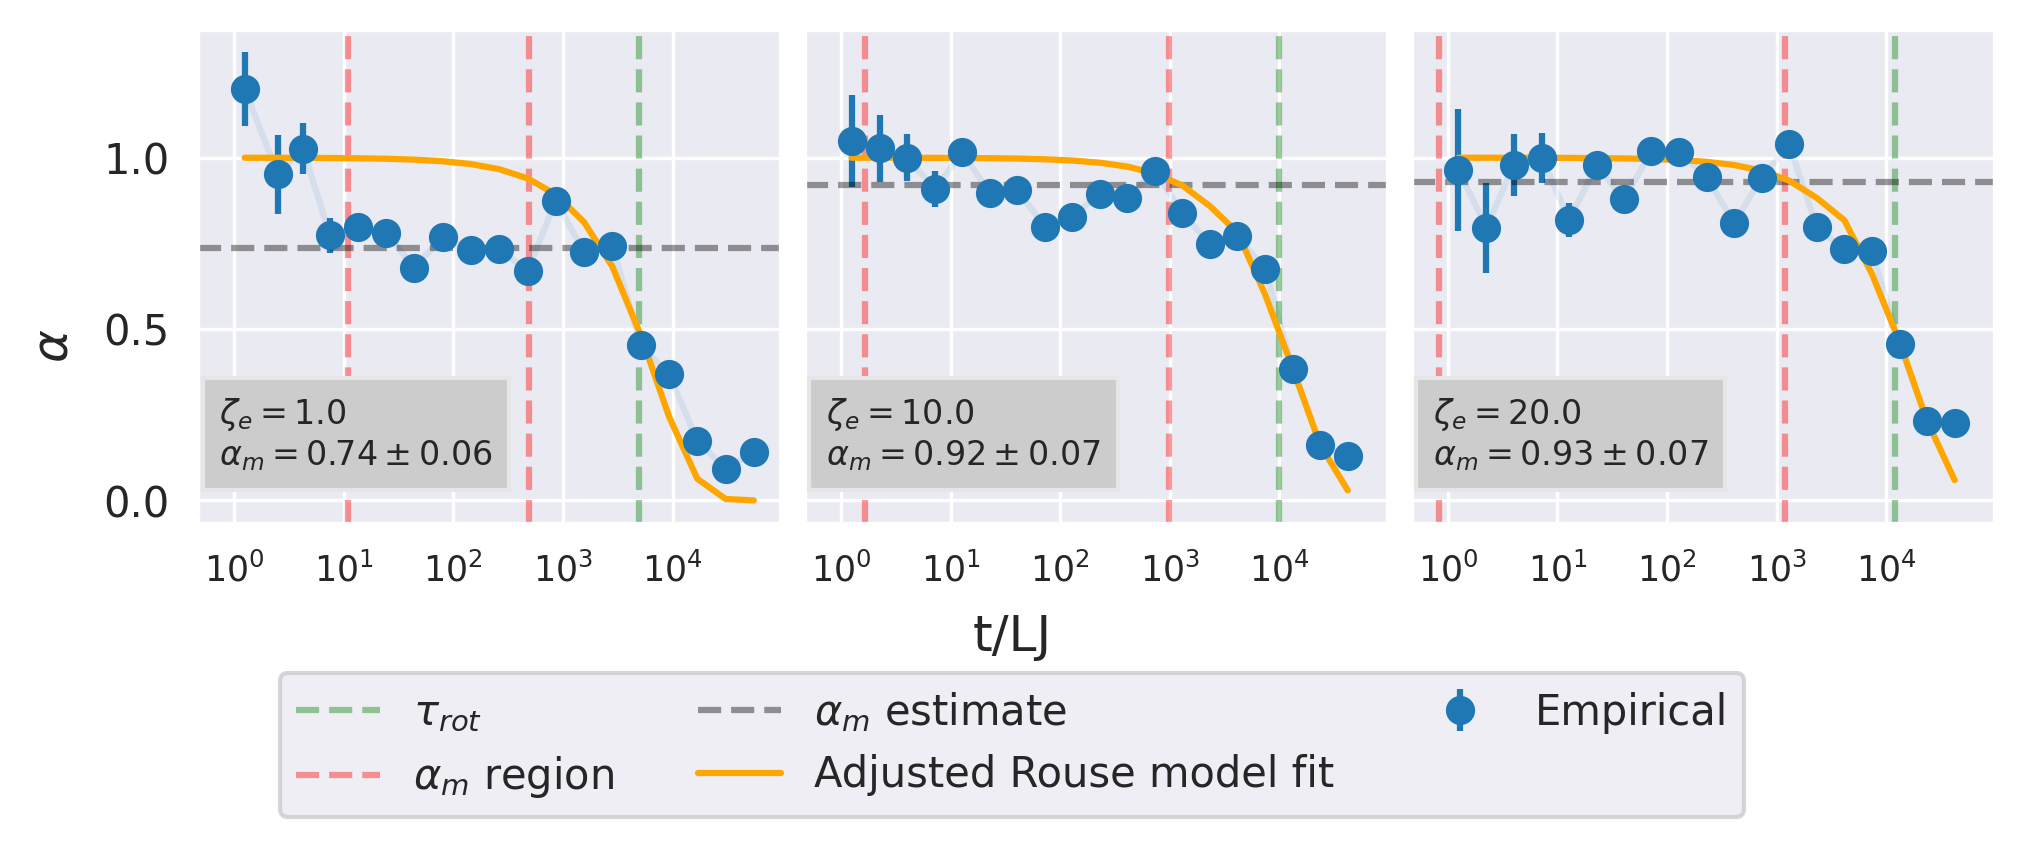
\includegraphics[width=\textwidth]{14+15+16-exp-alpha.png}
    \caption{Scaling exponent $\alpha$ of MSD of ETE 
    of anchored chains with different values of
    friction coefficient of the chain end $\zeta_e$ (blue dots);
    Scaling exponent $\alpha$ of corresponding fit
    of the Adjusted Rouse model (Eq.\ref{eq:adjusted_rouse_model_ete}, 
    orange line); Estimated scaling exponent for the time interval
    $t \ll \tau_{rot}$: $\alpha_m$ (grey dashed line); Red dashed lines
    correspond to $\alpha_m$ scaling region which is estimated as:
    $[10 \frac{m}{\zeta_e}, \frac{\tau_{rot}}{10}]$
    }
    \label{fig:alpha_anchored_zeta}
\end{figure}

\begin{figure}
    \centering
    \begin{subfigure}[b]{\textwidth}
        \centering
        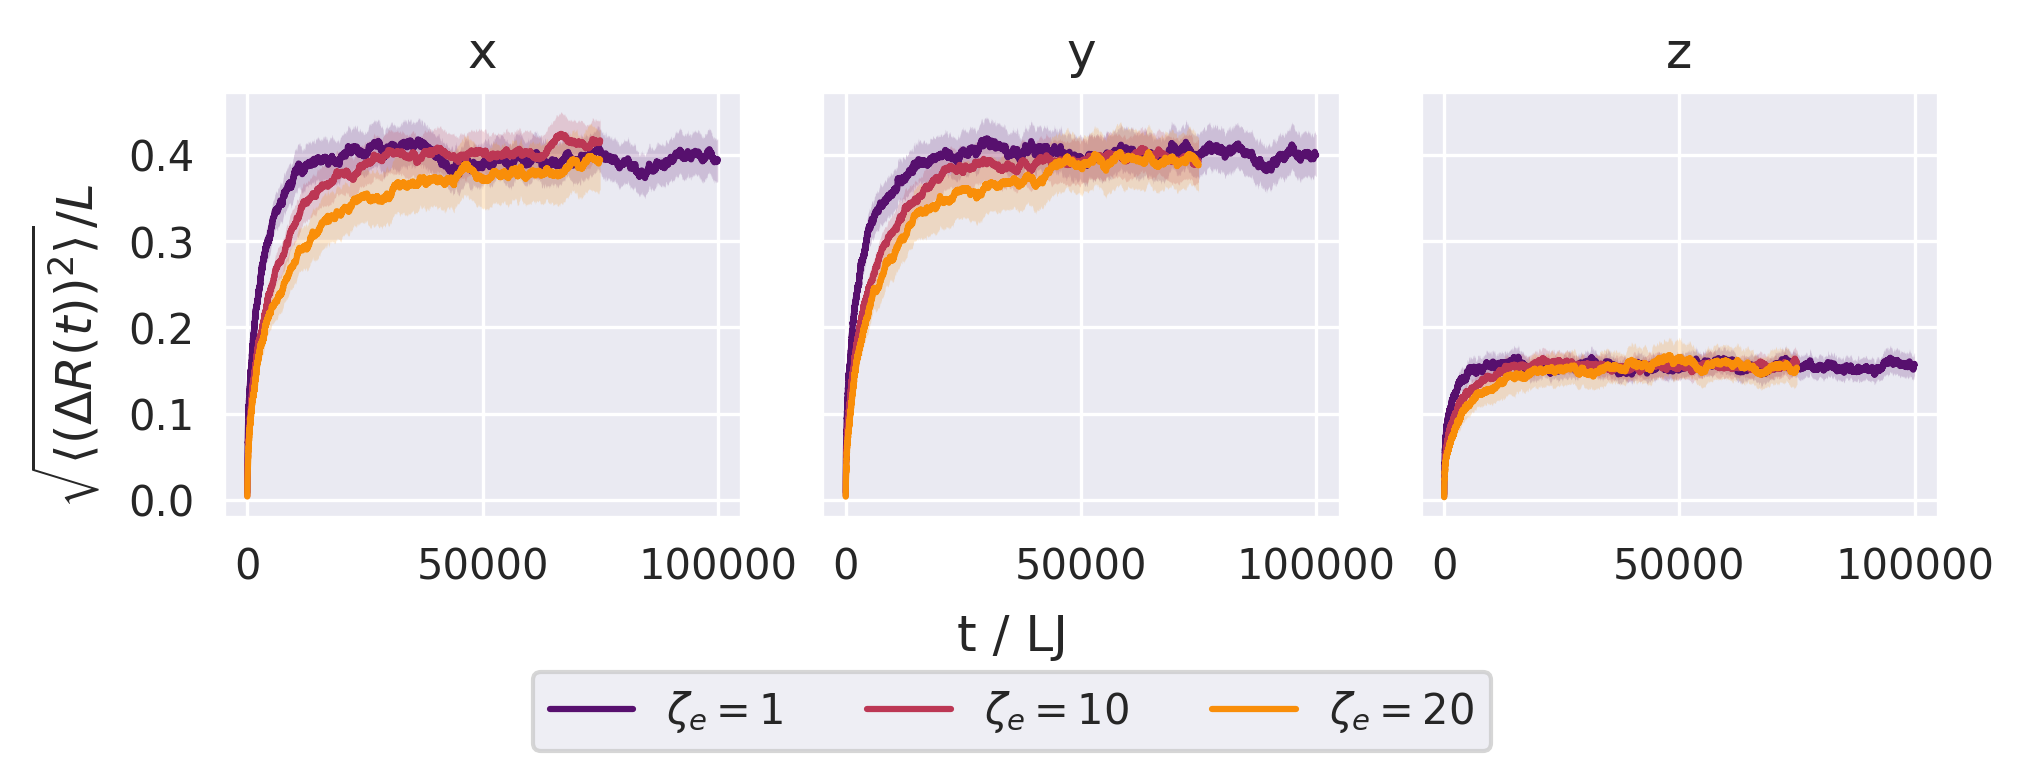
\includegraphics[width=\textwidth]{14+15+16-exp-msd-dim.png}
        \caption{normal scale}
        \label{fig:msd_anchored_zeta-dim-normal}
    \end{subfigure}
    \begin{subfigure}[b]{\textwidth}
        \centering
        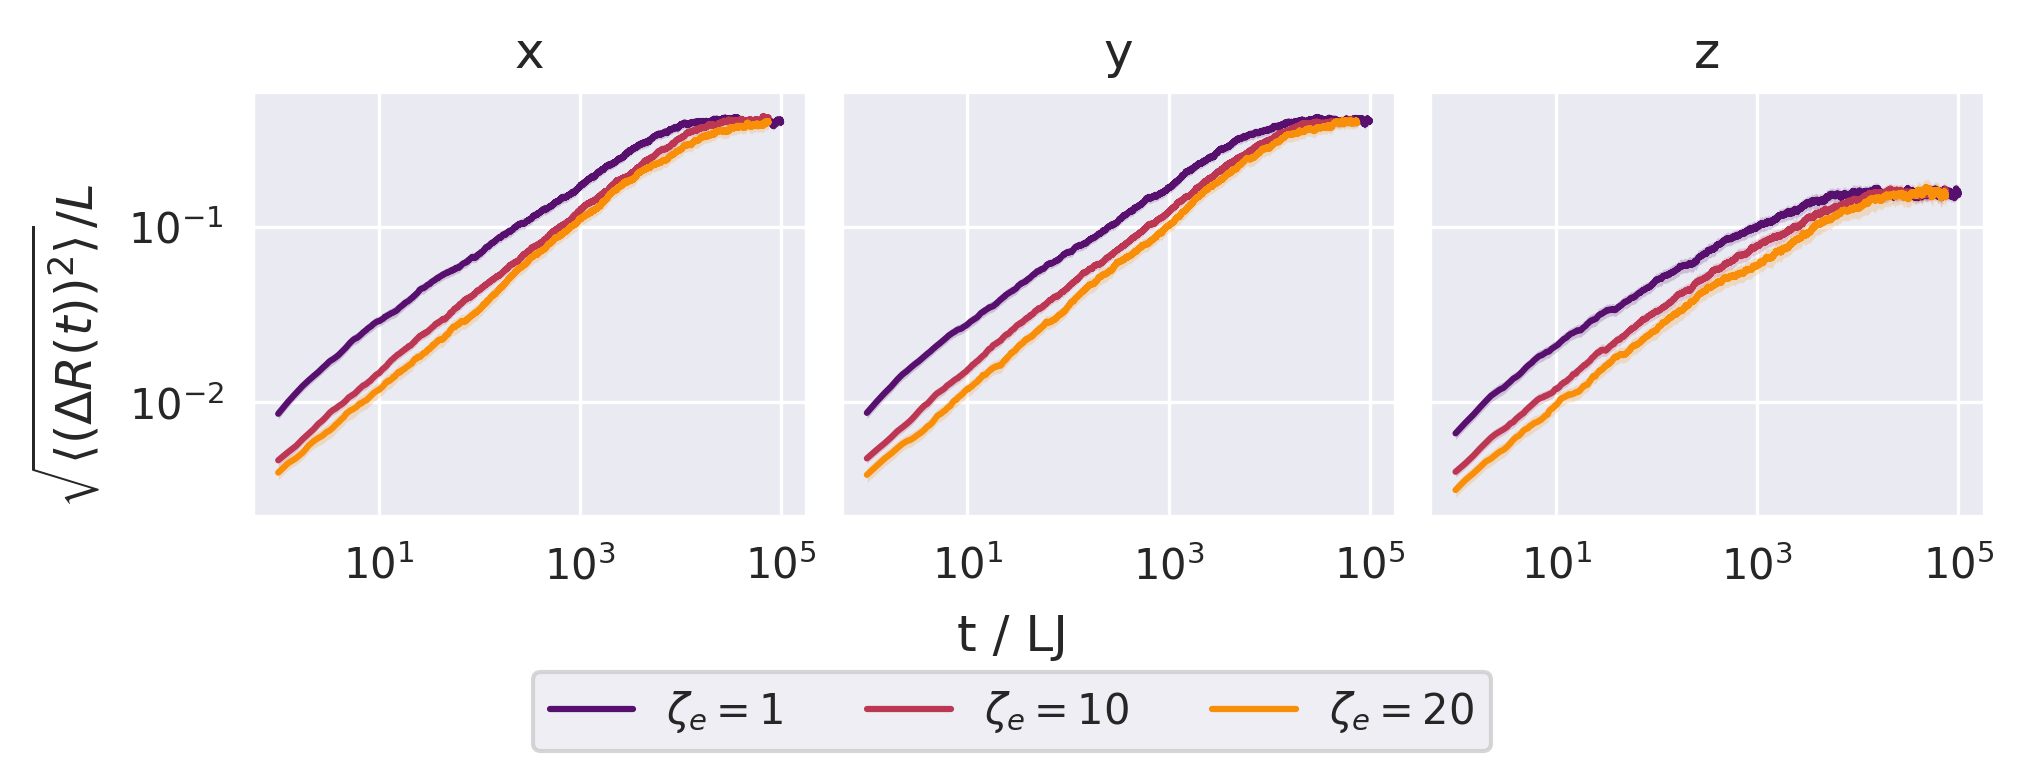
\includegraphics[width=\textwidth]{14+15+16-exp-msd-dim-log.png}
        \caption{log-log scale}
        \label{fig:msd_anchored_zeta-dim-log}
    \end{subfigure}
    \caption{
        Empirical MSD of ETE of anchored chains with different values of
        friction coefficient of the chain end $\zeta_e$ in main-axis system
        by dimension.
    }
    \label{fig:msd_anchored_zeta-dim}
\end{figure}

\FloatBarrier

\subsection{Free chain dynamics}
The following section focuses on the study of the dynamics of the 
free polymer chains. Specifically the the focus is on the verification
of the hypothesis arising from the discussion in the paper of 
Singh \emph{et. al.} \cite{Singh:2022}. Their work shows, that upon the 
binding of RAB5 to the EEA1 the scaling behavior of MSDLM in 
early time regime shifts from $3/4$ to the $2/3$. This behavior is explained
with the change of stiffness of the EEA1 upon the binding of RAB5, because
the scaling regime of MSDLM $\alpha=3/4$ corresponds the chains in the rod limit
and the $\alpha=2/3$ to the fully flexible chains in presence of excluded
volume interactions. The persistence length is estimated \emph{inderectly} by 
fitting the equation of MSDLM \cite{Singh:2022} derived in 
the Hinczewski \emph{et al.} \cite{Hinczewski_2009}. Therefore this approach does
not proove that change of scaling behavior is caused by exactly the change
of stiffness. An other factor possibly affecting the scaling behavior
is the increased friction coefficient of the end of the chain caused by 
bonded RAB5. Hence in this section the impact of the increased friction 
coefficient of the chain end ($\zeta_e$) on the scaling behavior of MSDLM is explored.
Additionally is checked if by changing the chain $l_p$ from the 
esimated for EEA1 value ($l_p/L_{\text{EEA1}} \approx 3.01$ \cite{Singh:2022}) to
the estimated for EEA1+RAB5 value 
($l_p/L_{\text{EEA1+RAB5}} \approx 0.3$ \cite{Singh:2022}) causes the 
similar to experimentally observed change of scaling behavior.
Some simplifications are made to reduce the computational resources
requirements and implementation complexity of simulation and analysis:
the number of beads of the chain is set to $N_b=64$ which results in 
contour length $L=61.11\text{LJ}$ which is smaller then the contour length of EEA1
$L_{\text{EEA1}}\approx222\text{nm}$.
\\
\\
The obtained MSDLM curves are shown on the \autoref{fig:msd_free}, the 
estimated scaling behavior on the \autoref{fig:alpha_free} and the 
corresponding $\alpha_{min}$ values are available in \autoref{table:free_chain_alpha_estimations}.
For the plausibility check the estimated scaling behavior of full flexible free chain is
displayed on \autoref{fig:alpha_free_full_flex}. 
\\
\\
Firstly, the $\alpha_{min} \approx 0.727$
in case $l_K/L=6.02$ approaches the expected value for the chain in the rod limit ($3/4$) 
and the $\alpha_{min} \approx 0.5$ (\autoref{fig:alpha_free_full_flex}) in 
case of the full flexible chain matches  almost exactly the expected value 
($1/2$), which is a good hint towards the results plausibility.
\\
\\
Secondly, the drop of $\alpha_{min}$ observed 
($0.727\pm0.001 \rightarrow 0.659\pm0.002 \Rightarrow \Delta\approx0.068$) by transition from $l_K/L=6.02$
to the $l_K/L=0.6$. 
Surprisingly both values are very close (however outside of CI) to the ones
of Singh \emph{et al.} \cite{Singh:2022}.
However, in case $l_K/L=0.6$ the $\alpha_{min}$ is 
far larger then $a_{min}$ of full flexible chain in contrast with the results
of Singh \emph{et al.} \cite{Singh:2022} where the $\alpha_{min}=2/3$ match 
the one of full-flexible chain, taking into account the presence of 
excluded volume interactions.
\\
\\
Thirdly, it is observed, that 
increased $\zeta_e$ causes non-neglible increase of $\alpha_{min}$:
\begin{itemize}
    \item In case $l_K/L=6.02$: $0.727 \pm 0.001 \rightarrow 0.803 \pm 0.001$ $\Rightarrow$ $\Delta\approx0.076$
    \item In case $l_K/L=0.6$: $0.659 \pm 0.002 \rightarrow 0.775 \pm 0.001$ $\Rightarrow$ $\Delta\approx0.116$
\end{itemize}
Given also the MSDLM curves in \autoref{fig:msd_free}, the one can conclude,
that the change in $\zeta_e$ affects the dynamics of the chains which is reflected in
the bahavior of MSDLM. Therefore when using the fit of analytical expression of MSDLM
to the empirical MSDLM to estimate some properties of the chain, one needs to account
for increased $\zeta_e$ to obtain more precise estimates.


\begin{figure}
    \centering
    \begin{subfigure}[b]{\textwidth}
        \centering
        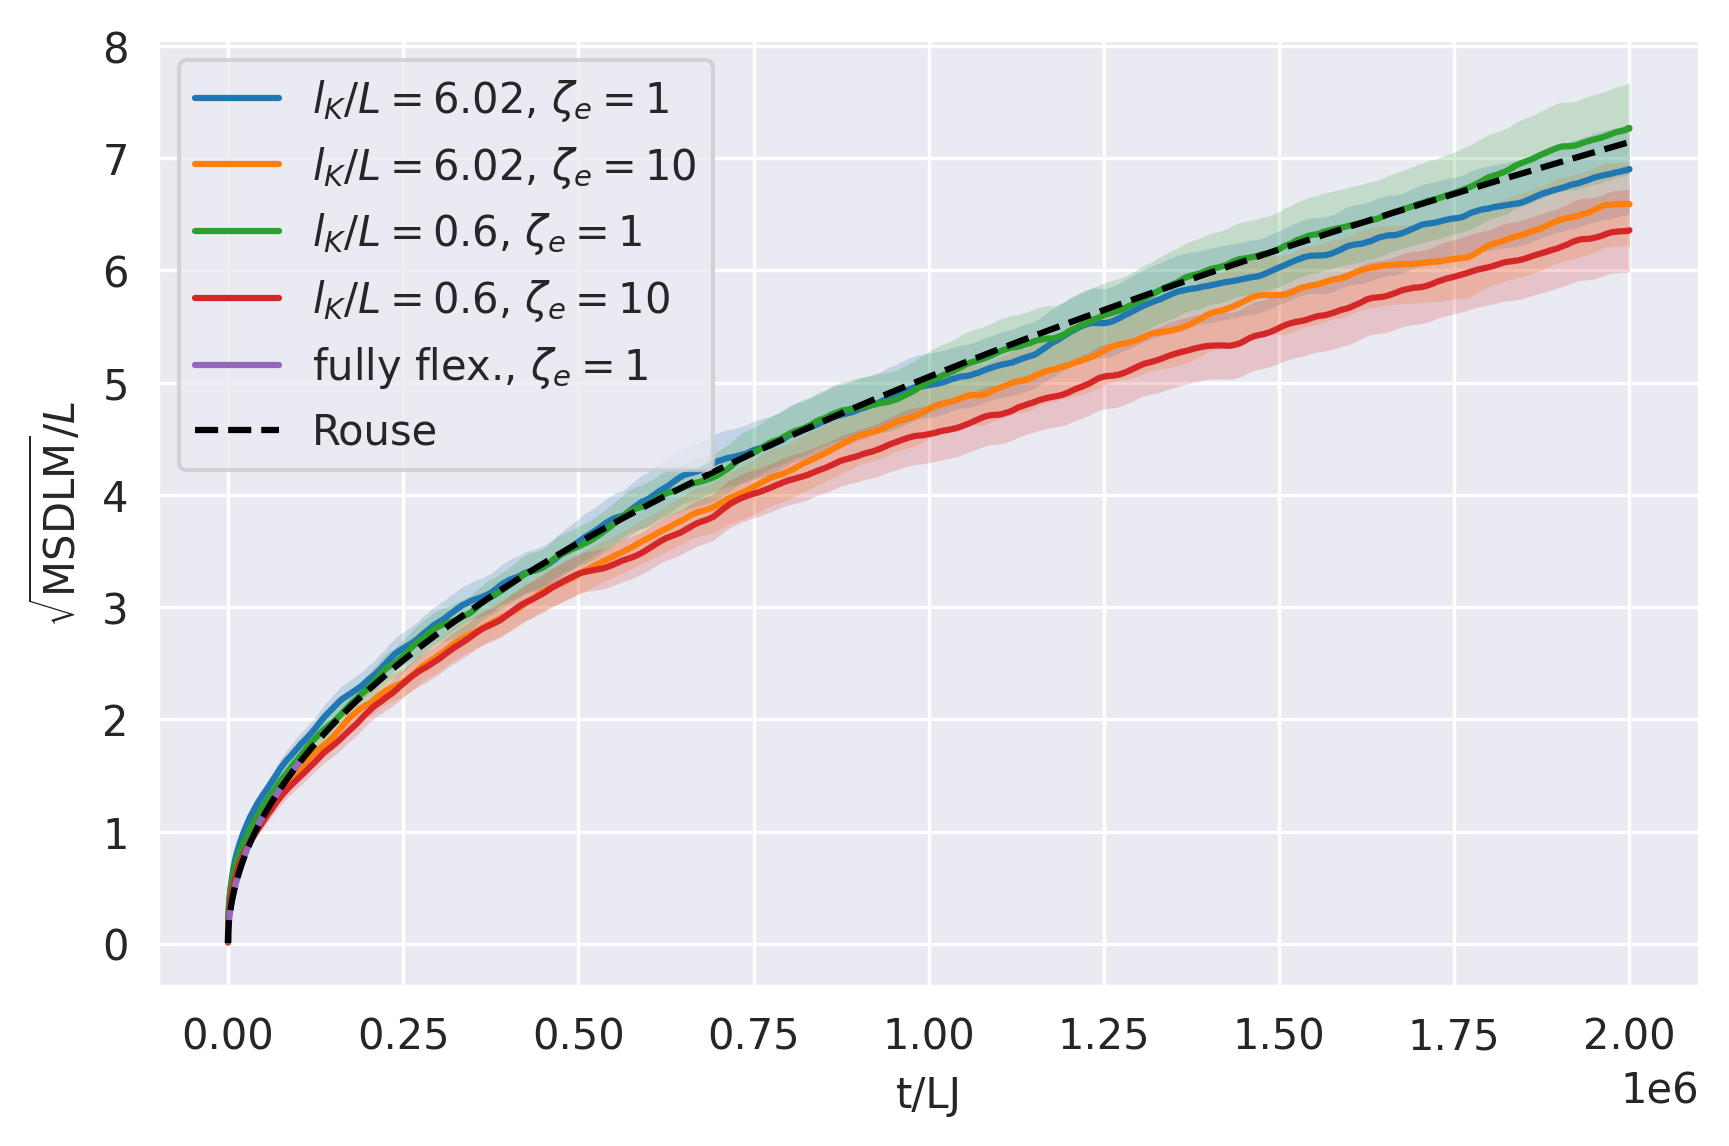
\includegraphics[width=\textwidth]{17+18+19+20-exp-msd.png}
        \caption{normal scale}
        \label{fig:msd_free-normal}
    \end{subfigure}
    \begin{subfigure}[b]{\textwidth}
        \centering
        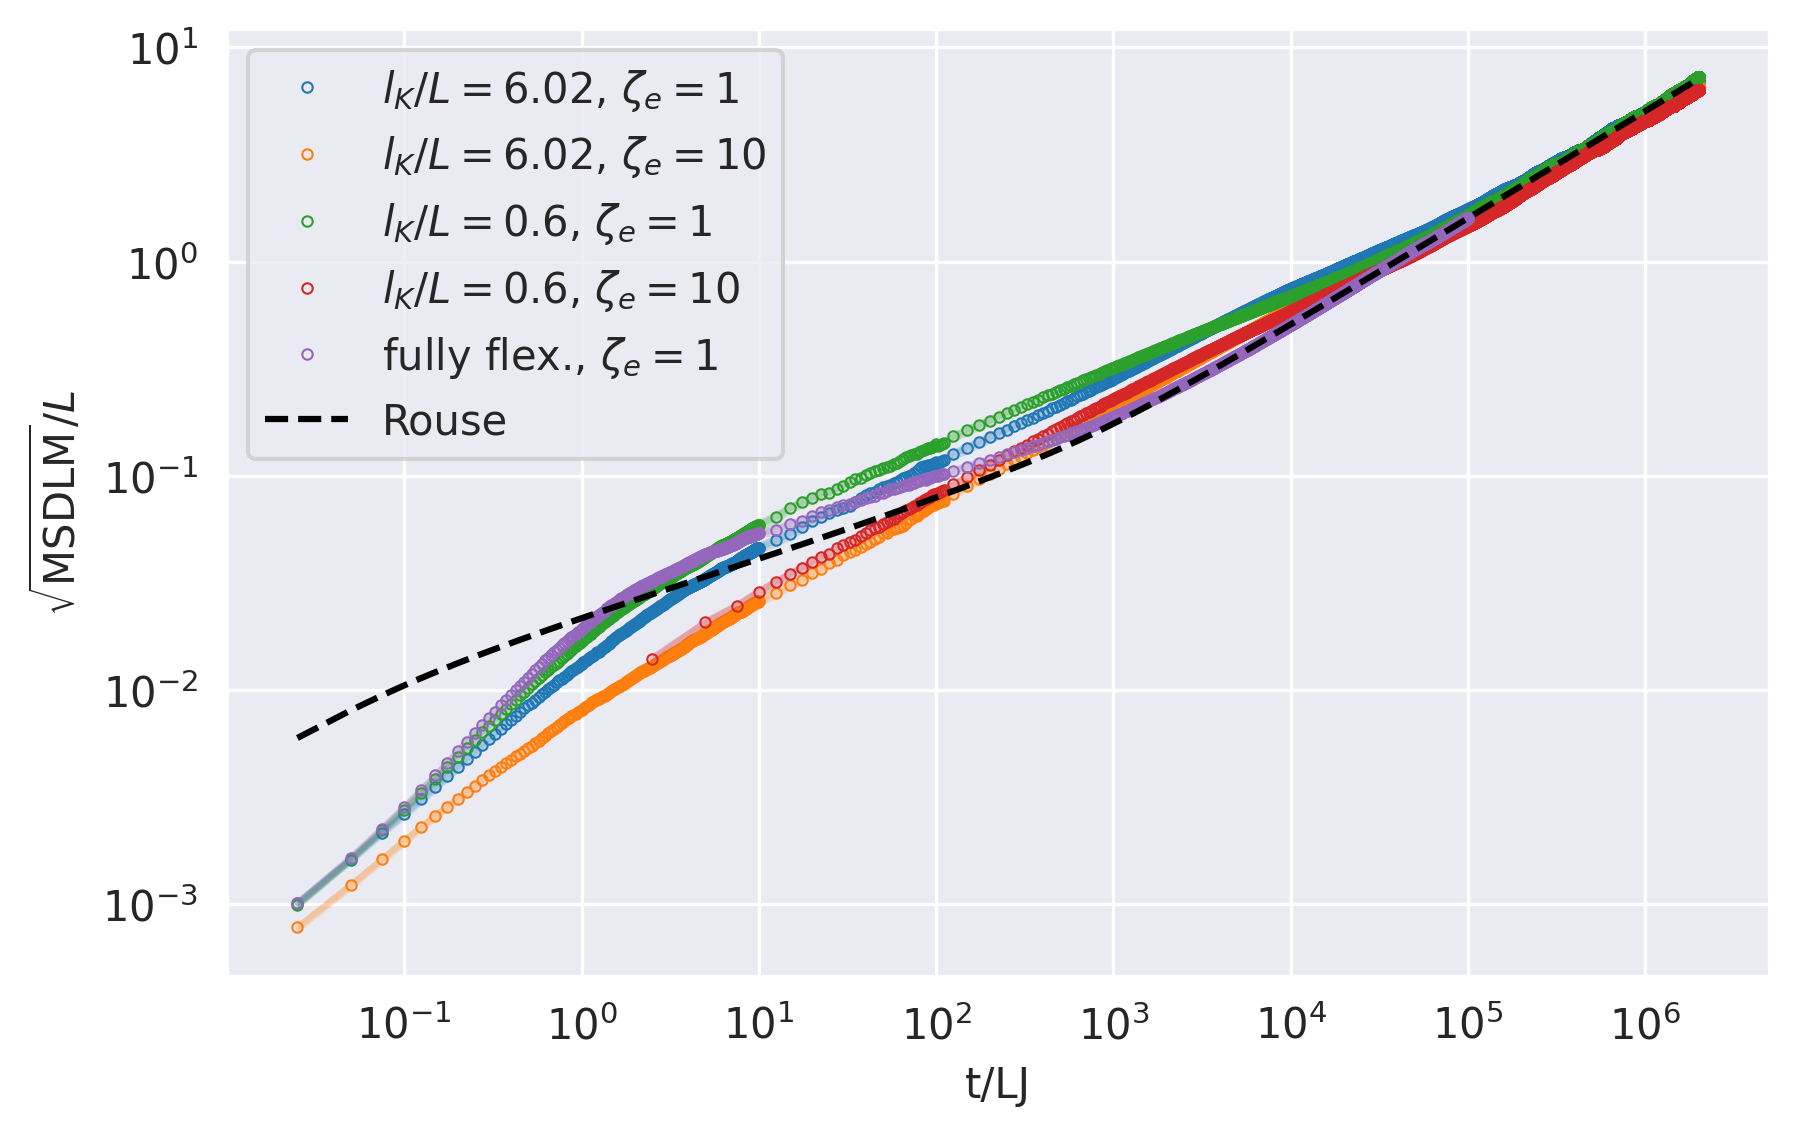
\includegraphics[width=\textwidth]{17+18+19+20-exp-msd-log.png}
        \caption{log-log scale}
        \label{fig:msd_free-log}
    \end{subfigure}
    \caption{
        Empirical MSD of chain end (MSDLM) of free chains
        with different stiffness and end-bead friction values and
        Rouse model prediction for fully flexible chains.
    }
    \label{fig:msd_free}
\end{figure}

\begin{figure}
    \centering
    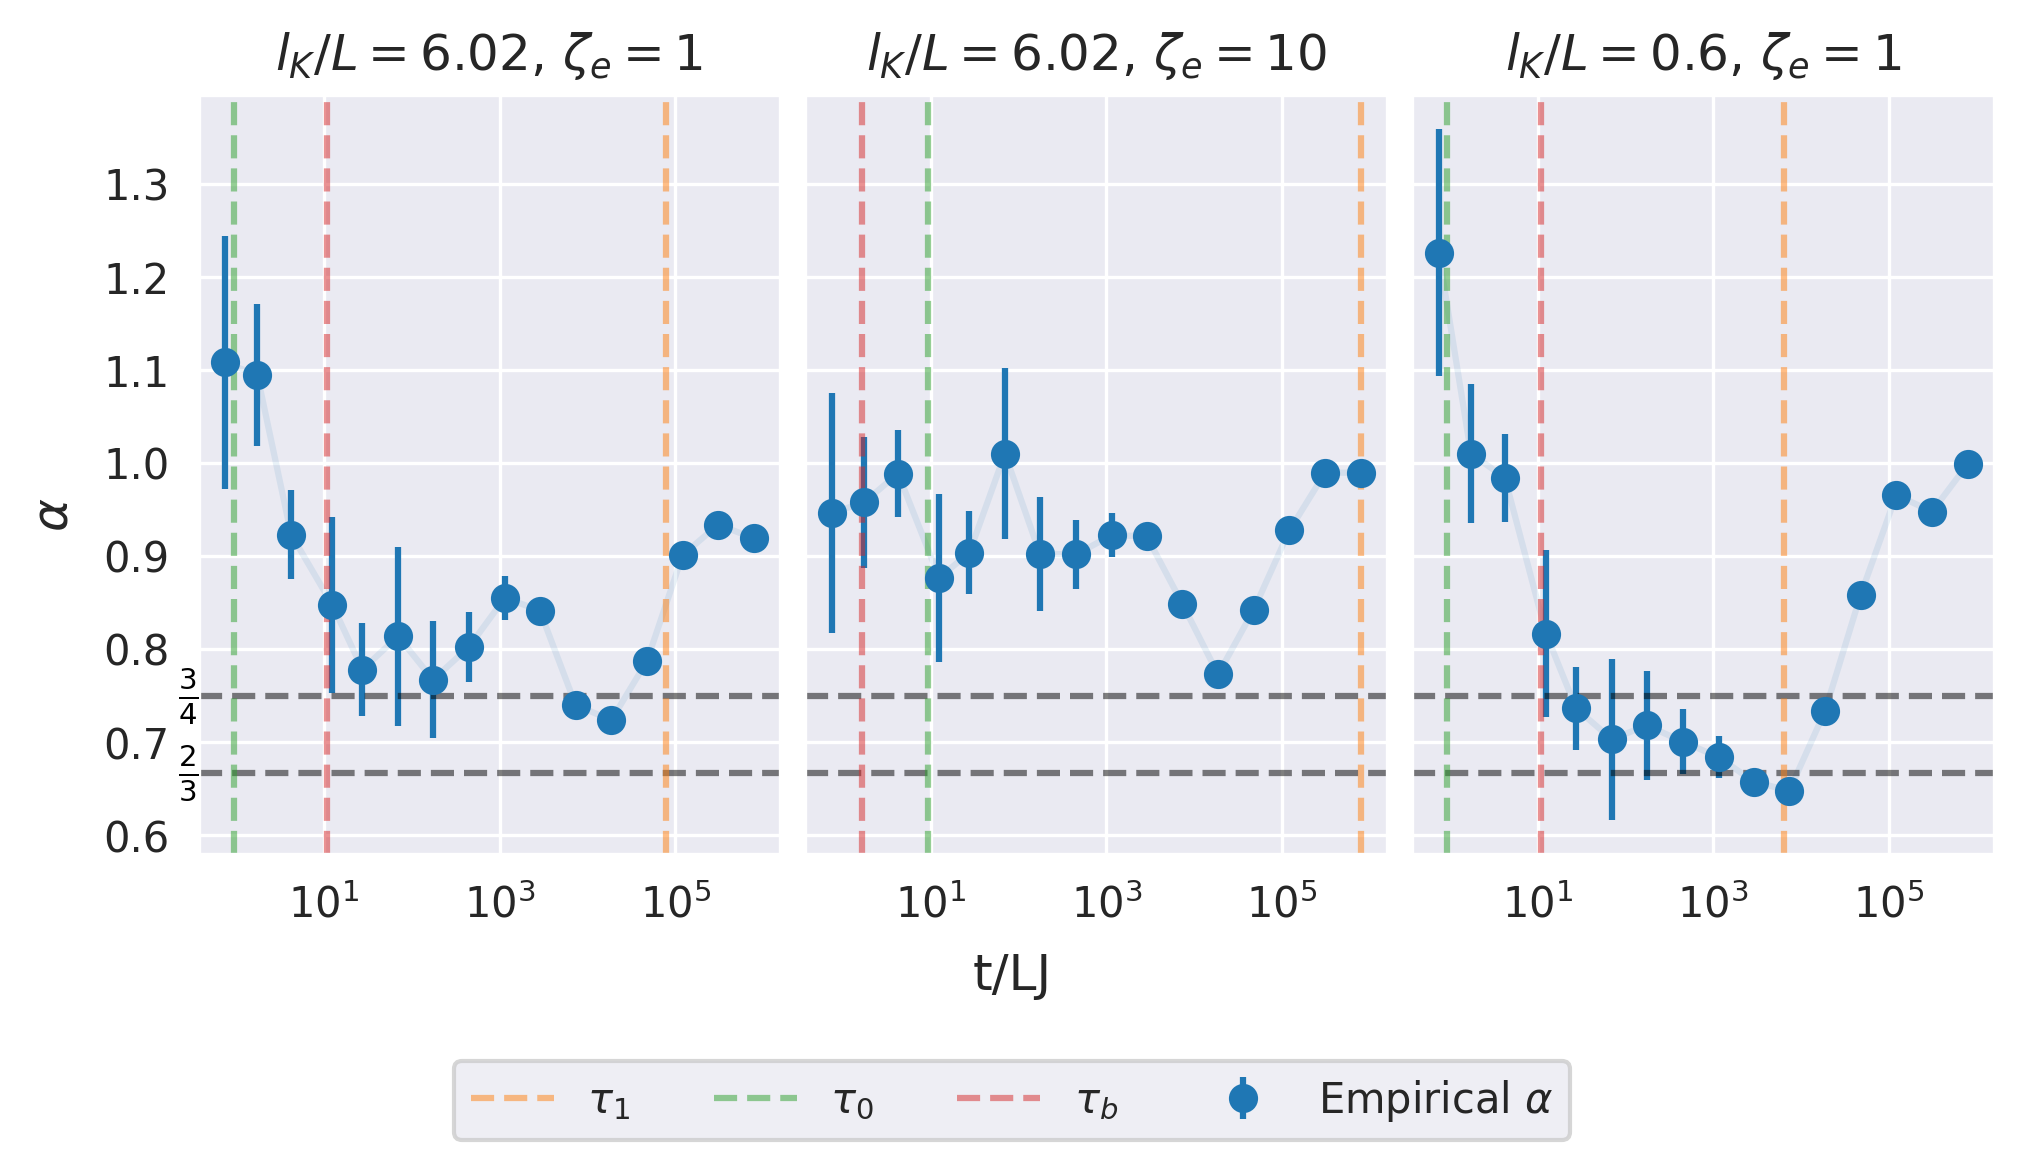
\includegraphics[width=\textwidth]{17+18+19+20-exp-alpha.png}
    \caption{Scaling exponent $\alpha$ of MSD of chain end (MSDLM) 
    of free chains with different stiffness and end-bead friction values;
    Grey dashed lines correspond to $3/4$, $2/3$, $1/2$ values.
    }
    \label{fig:alpha_free}
\end{figure}

\begin{figure}
    \centering
    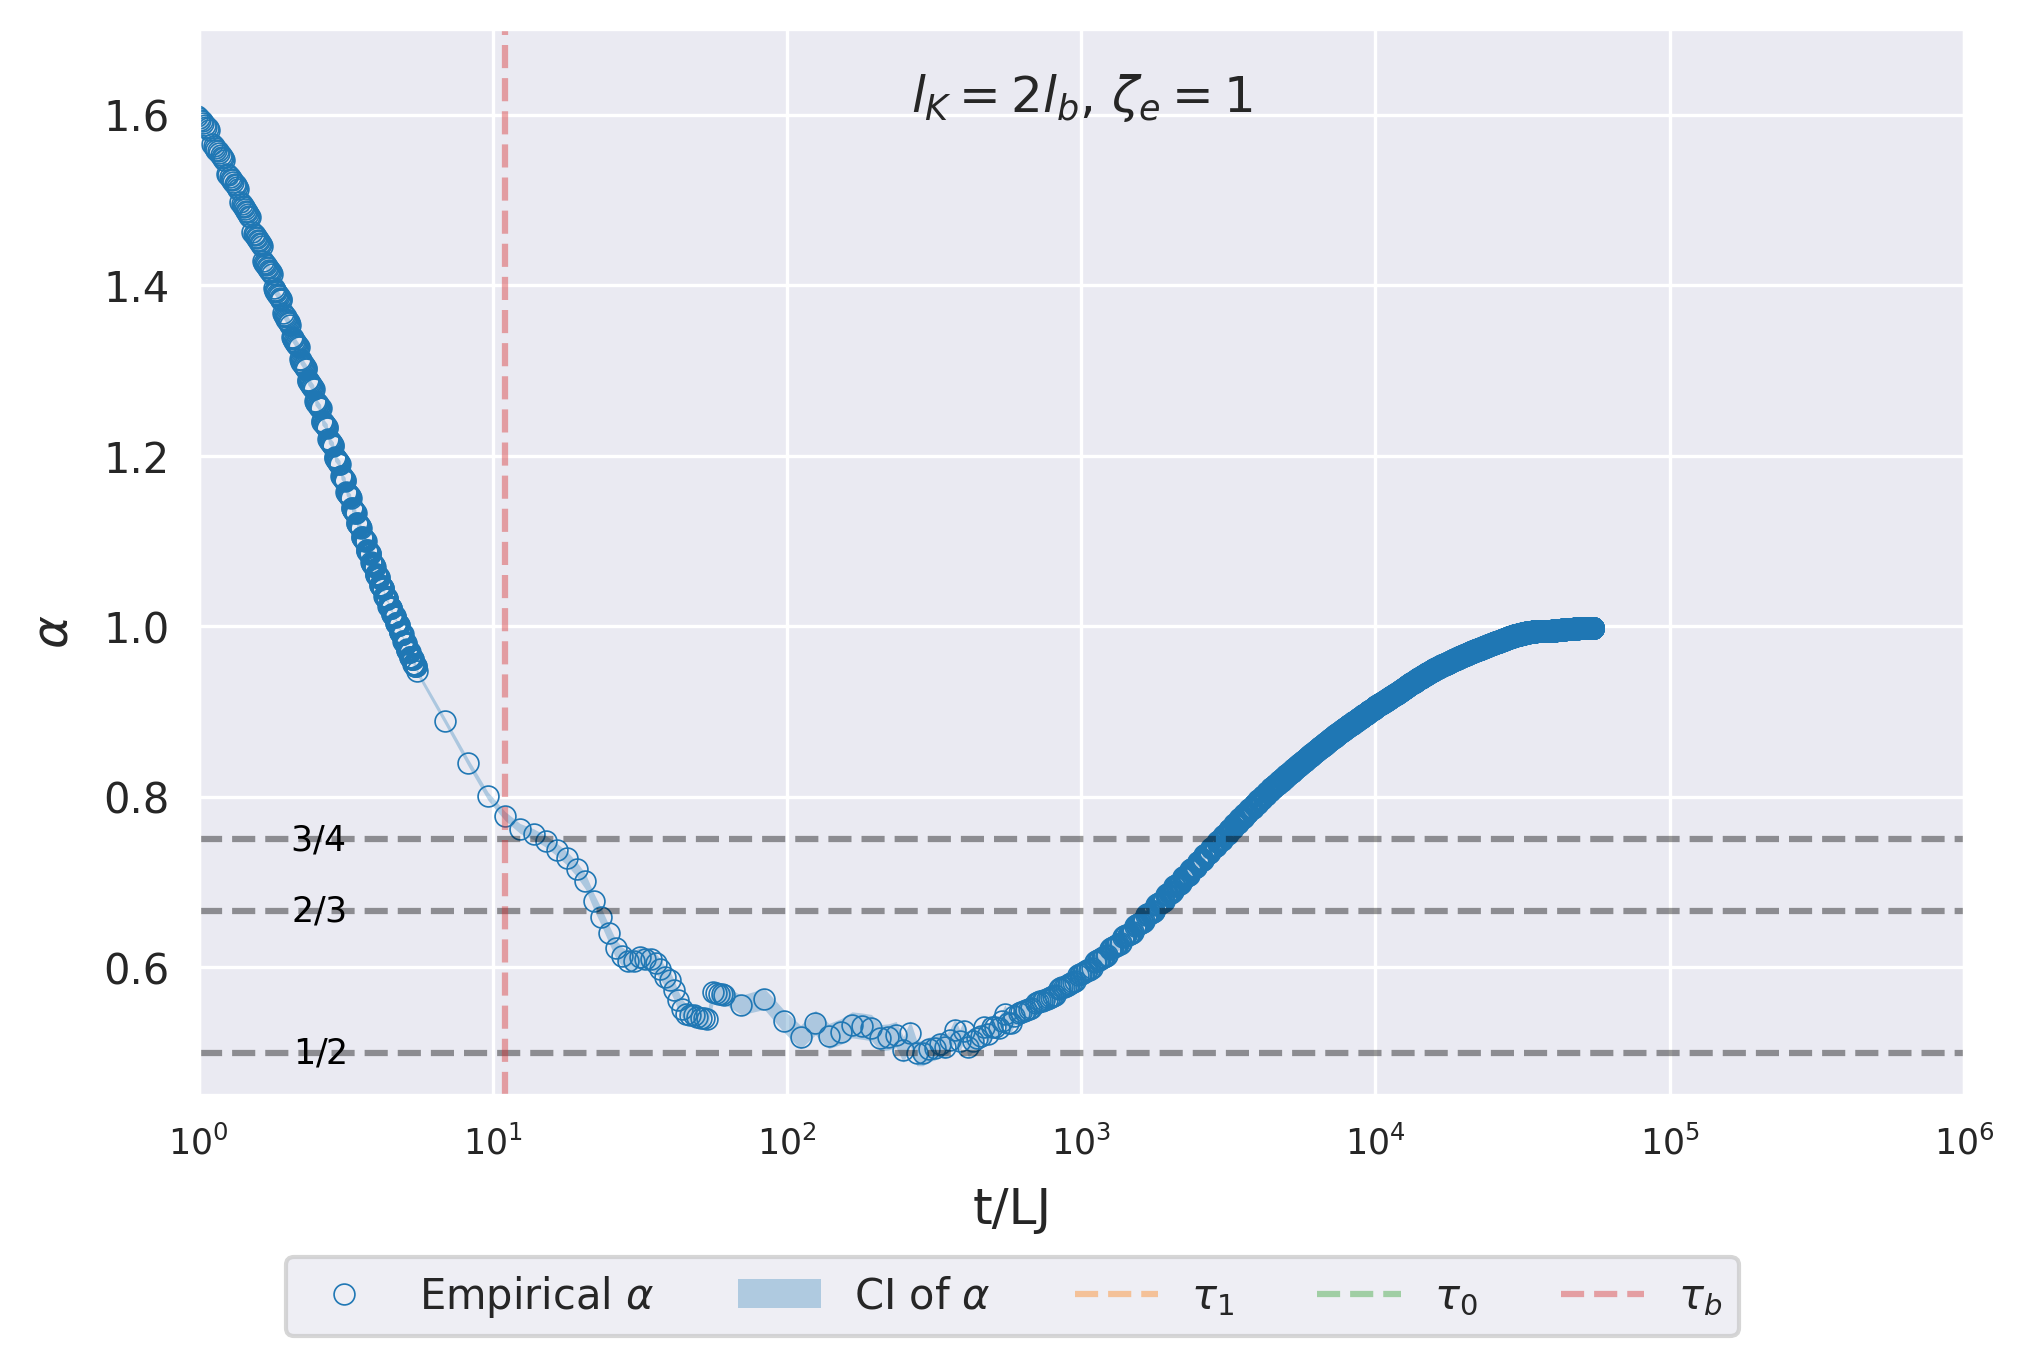
\includegraphics[width=\textwidth]{17+18+19+20-exp-full-flex-alpha.png}
    \caption{Scaling exponent $\alpha$ of MSD of chain end (MSDLM) 
    of free full flexible chain. $\tau_0$ and $\tau_b$ are outside of the
    x-axis boundaries. Estimated $\alpha_{min}=0.499 \pm 0.015$.
    }
    \label{fig:alpha_free_full_flex}
\end{figure}

\begin{table}[p]
    \centering
    
    \begin{tabular}{rrlllrrr}
        \toprule
        $\zeta_e$ & $l_K/L$ & $\tau_1$ & $\tau_b$ & $\tau_0$ & $\alpha_{min}$ & $\Delta \alpha_{min}$ \\
        \midrule
        1 & 6.02 & 78162.53 & 11.00 & 0.94 & 0.727 & 0.001\\
        10 & 6.02 & 781625.32 & 1.65 & 9.41 & 0.803 & 0.001\\
        1 & 0.6 & 6352.27 & 11.00 & 0.94 & 0.659 & 0.002\\
        10 & 0.6 & 63522.69 & 1.65 & 9.41 & 0.775 & 0.001\\
        \bottomrule
        \end{tabular}
    \caption{
        Free chains with different stiffness and end-bead friction values: 
        Estimated values of the minimum of the scaling exponent $\alpha$ and
        characteristic time scales.
    }
    \label{table:free_chain_alpha_estimations}
\end{table}

\section{Summary and Outlook}
In conclusion, the goals of this work are partially achieved. Multiple simulations 
are performed varying the chain stiffness and friction coefficient of the chain end, 
ignoring the hydrodynamic interactions. Resulting trajectories are processed and 
carefully analyzed. 

\paragraph{Anchored chains}
The specific dynamical quantity MSD of ETE (in following: MSD) was considered.
\\
\\
It is shown,
that the relaxation of free full flexible chain is faster then the one of
anchored ($\tau_{R,\text{free}} < \tau_{R,\text{anchored}}$). The Rouse model predictions
for free full flexible chains hold for anchored full flexible chains, if one considers
$\tau_R$ as free parameter. The estimation of $\tau_R$ for anchored full flexible chain 
delivers the correction factor for $\tau_R$ to account for anchoring.
\\
\\
In case of semiflexible chain several conclusions are made. As expected,
Rouse model predictions for flexible chains quickly diverge with observations made 
for semiflexible chains even with small stiffness ($l_p/L \approx 0.15$).
It is shown, that MSD of anchored semiflexible chains, 
similar to the case of full flexible chains, obeys the same 
proportionality ($\propto \exp\left(-\frac{t}{\tau_{rot}}\right)$) 
as anchored semiflexible chains for longer time scales, however with
different values of characteristic time $\tau_{rot}$. These characteristic times 
$\tau_{rot}$ are estimated for different values of stiffness. It was observed, that 
$\tau_{rot}$ grows with increasing stiffness of the chain. To explore the shorter time
scales the scaling exponent $\alpha$ of MSD is computed. In the region of subdiffusive 
motion with $t\ll\tau_{rot}$ the values of scaling exponent $\alpha$ match
qualitatively the expected ones for the minimum of scaling exponent in case of free chains.
Furthermore, the MSD was considered in different dimensions in "main-axis" coordinate 
system (Section \ref{sec:main-axis}). It is shown, that the difference with $z$ 
dimension increases with growing $l_p$, specifically, MSD in $z$ dimension is 
characterized through smaller relaxation time and lower value in long time limit.
\\
\\
Further the impact of the friction coefficient of chain end ($\zeta_e$) 
on dynamical properties of semiflexible chain in rod limit was studied.
The specific value of $l_p/L=3.01$ was selected to match the stiffness of
EEA1. Similarly to the study of impact of chain stiffness, it is shown,
that proportionality ($\propto \exp\left(-\frac{t}{\tau_{rot}}\right)$) holds
for $t>\tau_{rot}$ if $\tau_{rot}$ is considered as free parameter.
The increase of estimated $\tau_{rot}$ with rising $\zeta_e$ is observed.
The $\alpha(t)$ was calculated and the $\alpha$ value in the region of subdiffusive motion
(here called $\alpha_m$) was estimated. The small
increase of $\alpha_m$
($0.74 \pm 0.06 \rightarrow 0.92 \pm 0.07$) by the 
increase of $\zeta_e$ from $1$ to $10$ was observed and no difference was observed
in case of $\zeta_e$ transition from $10$ to $20$. Additionally, different dimensions
of MSD were considered in "main-axis" coordinate system, however, the effects of 
increased $\zeta_e$ are shown to be vizually consistent across the different dimensions.

\paragraph{Free chains}
The specific dynamical quantity MSD of the chain end (in following: MSDLM) was 
considered. The scaling exponent $\alpha(t)$ of MSDLM was examined. 
It is observed, that $\alpha_{min}$ decreases from $0.727 \pm 0.001$ to $0.659 \pm 0.002$ 
by the change of $l_p/L=3.01$ to $l_p/L=0.3$ in case $\zeta=\zeta_e=1$.
Furthermore it is shown, that
by increasing the $\zeta_e$, the minimum of scaling exponent $\alpha_{min}$ is also 
significantly increased in both cases: rod like $l_p/L \approx 3.01$ (matches the 
estimate for EEA1 in \cite{Singh:2022}) and
coil like  $l_p/L \approx 0.3$ (matches the estimate for EEA1+Rab5 in \cite{Singh:2022}).
Therefore, taking into account the observed MSDLM curves, the conclusion is made,
that when using the fit of analytical expression of MSDLM to the empirical MSDLM 
to estimate some properties of the chain, one needs to account
for increased $\zeta_e$ to obtain more precise estimates.

\paragraph{Outlook}
There are several limitations of this work, which can be improved in the future research.
Firstly it is necessary to increase the chain contour length $L$ to better match both the
theoretical requirement $l_b \ll L$ and the length of EEA1 chain. Then, the improvement 
would be to consider a grid of $l_p$ and $\zeta_e$ values to obtain the 
curves of characteristic times and $\alpha_{min}$ values in dependence of 
$l_p$ and $\zeta_e$. Of specific interest is the value of $\zeta_e$ which matches 
the value of real Rab5 bound to the end of EEA1. Finally, one needs to
consider hydrodynamic interactions, which may have significant impact on the dynamical
properties.  


% Erklärung
\clearpage
\thispagestyle{empty}
\minisec{Erklärung}\vspace*{1.5em}

Hiermit erkläre ich, dass ich diese Arbeit im Rahmen der Betreuung am Institut
für ??? Physik ohne unzulässige Hilfe Dritter verfasst und alle Quellen als solche gekennzeichnet habe.

\vspace*{45em}

Vorname Nachname \par
Dresden, Monat 2019

\bibliographystyle{plain}
\bibliography{sources}

\end{document}
